\documentclass[conference]{IEEEtran}
\IEEEoverridecommandlockouts
% The preceding line is only needed to identify funding in the first footnote.
% If that is unneeded, please comment it out.
% Template version as of 6/27/2024

\usepackage{cite}
\usepackage{amsmath,amssymb,amsfonts}
\usepackage{algorithmic}
\usepackage{graphicx}
\usepackage{textcomp}
\usepackage{xcolor}
\usepackage{tabularx}
\usepackage{multirow}   % \multirow
\usepackage{array}      % p{} column tweaks (usually already loaded)
\usepackage{booktabs}   % nicer tables (\toprule, \midrule, \bottomrule)
\usepackage{siunitx}    % consistent units, e.g. \SI{5}{\centi\meter}
\usepackage[hidelinks]{hyperref}

\graphicspath{{figures/}}

\definecolor{darkyellow}{RGB}{180,140,0}
\definecolor{darkgreen}{RGB}{0,150,20}

% Red TODO markers -- search for \todo before submission; none may remain.
\newcommand{\todo}[1]{\textcolor{red}{[TODO: #1]}}
\newcommand{\unsure}[1]{\textcolor{darkyellow}{[UNSURE: #1]}}
\newcommand{\bib}[1]{\textcolor{darkgreen}{[BIB: #1]}}
\newcommand{\Ttransform}[2]{\ensuremath{T_{\mathrm{#1}}^{\mathrm{#2}}}}
% Checkmark / dash for the comparison table
\newcommand{\cmark}{$\checkmark$}
\newcommand{\xmark}{--}

\begin{document}

\title{SCooP: A Real-World Indoor Multi-Robot Dataset for Collaborative SLAM and Perception over Measured Wireless Links\\

\thanks{Identify applicable funding agency here. If none, delete this.}
}

\author{%
\IEEEauthorblockN{Jorich Loquero and Ming-Chun Lee,~\IEEEmembership{Member,~IEEE}%
\thanks{The authors are with the Department of Electrical and Computer
Engineering, National Yang Ming Chiao Tung University, Hsinchu, Taiwan
(e-mail: jorich.ee14@nycu.edu.tw; \todo{email}).}}
}

\maketitle

\begin{abstract}
\unsure{Cooperative robotic systems must jointly solve perception, sensing, and
communication, yet existing datasets capture at most two of these layers at
once. We present SCooP, a multi-agent, multi-view, multi-sensor dataset that
spans all three: synchronized camera, radar, LiDAR, and RTK-GNSS sensing;
cooperative perception annotations; and measured, replayable wireless channel
traces. Each platform is spatially calibrated and temporally aligned, enabling
tasks across single-agent and collaborative scenarios and modalities. We
provide ground-truth poses, TSDF reconstruction supervision, RSSI channel
traces, and object annotations, together with benchmarks for cooperative
perception under clean and actual channels, point cloud reconstruction, and
cross-modal localization. \todo{One sentence with the headline result, e.g.
``Cooperative perception improves mAP by X points over single-agent, and the
logged channel reduces this gain by Y.''} The dataset and development kit are
publicly available at \todo{URL/DOI}.}
\end{abstract}

\begin{IEEEkeywords}
multi-agent systems, cooperative perception, collaborative SLAM, integrated
sensing and communication, dataset, benchmark
\end{IEEEkeywords}

%=======================================================================
\section{Introduction}
\label{sec:introduction}
Collaborative robotic systems --- fleets of vehicles, drone swarms, and
multi-robot teams --- depend on three tightly coupled layers: \emph{sensing}
for localization and mapping, \emph{perception} for scene understanding, and
\emph{communication} for sharing information between agents. In a robot team these layers meet in two processes: collaborative
SLAM (C-SLAM), which places every robot in one shared map
\cite{swarmslam,doorslam}, including its metric-semantic variants
\cite{kimeramulti}; and collaborative perception, which fuses what
the agents observe within that map, from object detection to semantic
scene understanding \cite{where2comm}. 

Collaboration promises multiple improvements on single-agent scenarios such as
occlusion handling and faster coverage but this can only be realized when the
three layers are handled together. For example, a neighbor's detection is
useful only if it arrives before the scene changes and can be placed in the
receiver's frame with accuracy comparable to its own sensors. This requires circumventing a communication constraint on a real wireless link and a localization constraint more challenging in indoor scenarios.

Existing collaborative datasets above are outdoor relying ground truth vehicle and infrastructure poses come from RTK-GNSS \cite{dairv2x,deepsense6g,v2v4real},
and multi-robot trajectories from GNSS- or total-station-assisted SLAM
\cite{kimeramulti}. Indoor environments, where cooperation matters most
as occlusion is dense, line of sight is short, and the wireless channel is
dominated by multipath are also where GNSS is
unavailable, so the reference every outdoor dataset relies on does not exist.
Existing indoor datasets consequently trade coverage for accuracy: motion
capture is confined to an instrumented volume \cite{utias,m2dgr}, sparse anchors
leave odometry to carry the pose between them \cite{hilti2022,airmuseum},
endpoint-only labeling never records the interior of a trajectory \cite{s3e},  map registration presupposes an onboard LiDAR and provides no external check where the geometry is degenerate
\cite{subtmrs} and some releases report the estimator's own pose with no independent reference at all \cite{coped}.

Furthermore, these datasets cover these layers only partially. Collaborative SLAM
datasets provide rich synchronized sensing but treat communication
implicitly \cite{s3e,kimeramulti,coped}; cooperative perception
benchmarks provide labels while idealizing or simulating the channel
\cite{opv2v,dairv2x,v2v4real}; and joint sensing--communication datasets
log the real channel but offer no cooperative scene understanding, and do
so outdoors \cite{deepsense6g}. Measured indoor channel datasets
provide precise transmitter positions but no perception sensing and no
multi-agent structure \cite{dichasus}, while ray-traced alternatives
supply arbitrarily dense channel and pose samples at the cost of a
simulated propagation environment \cite{deepmimo}. As a result, two questions that span layers remain open: \emph{how much
perception accuracy a real indoor link costs}, and \emph{how much of that
cost could be anticipated from the geometry the agents already map}.
Neither can be answered with any single existing dataset.

We close this gap with \textbf{SCooP}: a multi-agent, multi-view,
multi-sensor dataset that jointly captures all three layers under
building-scale indoor ground truth. The main contributions of this
paper are:
\begin{itemize}
    \item \textbf{A joint sensing and communication dataset with indoor ground truth.}
    Synchronized LiDAR, camera, IMU, and mmWave radar from three mobile and two
    infrastructure agents, with each frame carrying the measured link state,
    channel state, and clock offset of every agent pair. All agents, including an RGB-D-only robot, are placed in one metric
    frame by registration against a self-built reference map, validated
    against independent control distances; 3D boxes, per-point labels,
    and rendered masks are expressed in the same frame.
   \item \textbf{Characterized trajectory paradigms.}
    Concurrent, intersecting, and rendezvous runs whose occlusion, co-visibility, viewpoint diversity, and Fresnel link clearance are computed per frame from the reference map and validated against measurements they do not use. These quantities serve as predictors of where collaboration will degrade, testing how much of the link's cost could be foreseen from the geometry alone.
   \item \textbf{Benchmarks.} Collaborative SLAM (C-SLAM) and collaborative perception baselines under idealized, synthetic, and measured channels, reporting the accuracy the link costs and the share of that cost the geometry anticipates.
\end{itemize}

%=======================================================================
\section{Related Work}
\label{sec:related}
We review prior datasets against the two questions of Sec.~I. Measuring
what a real link costs requires the channel recorded on the sensing
timeline, together with ground truth for every agent throughout its
trajectory. Testing whether that cost could be foreseen from mapped
geometry further requires the geometry to be released per frame and
computed independently of the signal it is meant to predict.

\subsection{Collaborative SLAM Datasets}
Multi-robot SLAM datasets provide synchronized multi-agent sensing for
collaborative localization and mapping.
SubT-MRS~\cite{subtmrs} extends multi-robot recordings to degraded
underground and all-weather conditions. The Kimera-Multi
datasets~\cite{kimeramulti} cover campus-scale outdoor sequences
with up to eight robots, and S3E~\cite{s3e} adds UWB inter-robot
ranging and four trajectory paradigms designed around intra- and
inter-robot loop closures. CoPeD~\cite{coped} and
CU-Multi~\cite{cumulti} move toward collaborative perception by
adding image-level semantics and larger multi-session coverage,
respectively. Across all of these, however, the communication layer
is absent or incidental: inter-agent links are either assumed ideal or
logged only as a by-product of the C-SLAM system under test, and no
channel measurements are released alongside the sensor streams. A
recent planetary-analogue C-SLAM dataset~\cite{planetary_cslam} is a
notable exception in reporting measured peer-to-peer latency and
throughput, but it provides no perception labels. In C-SLAM systems, communication is reported as the volume of
data exchanged \cite{doorslam,swarmslam}, not as the accuracy lost to
a measured link. What a real link costs C-SLAM therefore cannot be
measured on any of these datasets. SCooP differs in
recording the channel as a first-class stream on every link and in
pairing it with cooperative perception annotations. The same gap holds for semantic SLAM. The datasets on which it is
evaluated are single-agent, with indoor ground truth from motion
capture and outdoor ground truth from GNSS \cite{semslam_survey}; its
multi-robot extensions, which exchange object-level maps between
agents \cite{kimeramulti}, have no data with per-agent indoor ground
truth, object labels consistent across agents, or a measured link over
which the compactness of a semantic map could be tested.

\subsection{Cooperative Perception and Communication Datasets}
Cooperative perception benchmarks supply multi-agent labels for
detection and tracking, either in simulation
(OPV2V~\cite{opv2v}) or from real vehicles and
roadside units (DAIR-V2X~\cite{dairv2x}, V2V4Real~\cite{v2v4real}). Communication-efficient fusion methods such
as Where2comm~\cite{where2comm} are evaluated on these benchmarks
under fixed bandwidth budgets and synthetically injected latency or
packet loss, so the channel is abstracted rather than measured.
Two recent efforts begin to close this gap for driving:
V2X-ReaLO~\cite{v2xrealo} evaluates online fusion over a live Wi-Fi
link, and CooperScene~\cite{cooperscene} releases per-scene C-V2X
latency, throughput, and loss traces alongside multi-modal sensing
and 3D labels. Both are outdoor, vehicle-centric, and
single-scenario in their agent geometry and neither relates the loss observed to the scene geometry that produced it. SCooP targets the
complementary indoor multi-robot setting, with mobile agents whose
relative geometry and link state vary within a run, and with
building-scale pose ground truth against which perception and
reconstruction can be jointly evaluated.

\subsection{Joint Sensing--Communication Datasets}
Integrated sensing and communication (ISAC) datasets co-register
real wireless measurements with conventional sensors. DeepSense
6G~\cite{deepsense6g} synchronizes mmWave and sub-6\,GHz channel data
with camera, LiDAR, radar, and GPS across vehicular, drone, and
indoor scenarios, primarily for beam and blockage prediction.
DICHASUS~\cite{dichasus} provides massive-MIMO CSI with
sub-decimeter position ground truth for channel-based localization,
and DeepMIMO~\cite{deepmimo} offers ray-traced CSI for the same
tasks but in simulated settings. These datasets ground the communication layer in measurement but are single-link and task-agnostic with respect to
robotics: the transmitter follows a scripted path, no other agent
cooperates with it, and no scene-understanding labels are provided.
SCooP retains the measured-channel character of ISAC data while
embedding it in a multi-agent cooperative task with perception and
reconstruction supervision.

\subsection{Ground Truth for Indoor Multi-Agent Datasets}
A collaborative-perception benchmark places a heavier demand on its
reference than a SLAM benchmark does. In SLAM evaluation, the
reference is a target: an error in it perturbs a benchmark number.
In a perception dataset, annotations
are derived from and expressed through the reference poses, so any
error propagates into every label. This requires a pose for every
scan of every agent, expressed in one common metric frame so that
observations from different robots can be related. Indoor datasets
meet these demands to varying degrees, differing along two axes:
where the reference geometry comes from, and whether it is validated
\emph{independently}---against a higher-accuracy measurement that did
not inform the solution---or only by internal consistency.
\emph{Motion capture} handles multiple agents naturally and gives
millimeter-accurate, independently measured trajectories, but only
inside a camera-instrumented volume, typically a single room
\cite{utias,m2dgr}. \emph{Sparse anchoring} spreads surveyed
references across a site whether it be total-station control points
\cite{hilti2022} or fiducial beacons constraining a
structure-from-motion solution \cite{airmuseum} but between anchors
the pose is carried by odometry or SfM; taken to its limit, some
multi-agent releases provide full trajectories only within a short
mocap segment and endpoint poses elsewhere \cite{s3e}, leaving
sequence interiors, where inter-agent observation fusion
happens, unevaluated and unannotatable. \emph{Map registration}
aligns each scan to a dense prior of the whole site and yields full,
independently validated trajectories at building scale, including
multi-robot and multi-session releases \cite{subtmrs}
and even heterogeneous camera-centric devices in AR settings
\cite{lamar} but in every case the guarantee is inherited from a
prior captured with a dedicated survey scanner.
\emph{SLAM-derived pseudo-ground truth} dispenses with the survey
instrument: an offline SLAM solution supplies a pose for every scan.
Single-agent instances attaches quantitative
checks such as sparse physically measured landmark distances
\cite{incrowdvi} while
the multi-robot instances we are aware of validate by internal
consistency alone: overlay against geospatial imagery \cite{envodat}. Independent traversals can converge to the same wrong geometry, most likely in degenerate regions such as featureless corridors, where a converged registration offers no internal evidence of being correct. Notably, none of these references is used to derive labels
as the annotations these datasets carry, where present, are authored
independently of the reference poses. Finally, some multi-robot
releases report the estimator's own pose with no reference at all
\cite{coped}.

SCooP combines three of these strategies: an offline SLAM-derived map, scan-to-map registration against it, and fiducial anchoring
(Sec.~\ref{sec:gt}). Unlike prior SLAM-derived references, ours is
validated against independent control distances, cross-referenced between repeated passes and is used to derive the collaborative perception annotations.

\subsection{Collaboration Geometry in Multi-Agent Datasets}
\label{sec:geometry}

Asking how much of the link's cost could be foreseen from mapped
geometry treats collaboration geometry as a predictor. That requires
it to be released per observation, and computed independently of the
outcome it predicts. A collaborative-perception benchmark reports
accuracy obtained under a collaboration geometry, that is, which nodes
could see an object, how well, and from what relative viewpoint, yet
that geometry is seldom a released quantity. Datasets differ along two
axes: whether the geometry is deliberate, and whether it is measured
per observation or merely described.

Multi-robot SLAM datasets design their trajectories around loop
closures rather than shared views of objects. S3E~\cite{s3e} names four
collaborative trajectory paradigms and grades each against loop-closure
opportunity with filled and open circles, and CU-Multi~\cite{cumulti} treats inter-trajectory overlap as a controlled variable. The grading, however, is an assertion about a run rather than a quantity attached to a frame, and the overlap is obtained by re-running one platform four times, so no instantaneous geometry exists to measure; both, moreover, collaborate between sensors at a common height, leaving the elevated-to-ground asymmetry absent by construction.

In collaborative perception datasets, relative geometry
follows from how the collecting vehicles happened to drive, whether simulated \cite{opv2v} or recorded on public roads \cite{v2v4real}, or from sensor placement and the ego's approach at an instrumented site \cite{dairv2x}. Per-frame poses are necessarily released, feature warping depending on them, so relative placement is recoverable; what is absent is the condition itself---no
field states whether the ego's view of an object was blocked, whether a
partner's was clear, or at what angle the two observed it, and in the recorded sets no dense scene model accompanies the release from which to reconstruct it.
Splits are cut by town, road type, or scene, never by geometry, and where
geometry does enter it enters as a nuisance to be corrected: pose error is
modelled, injected, and compensated, while the geometry that error perturbs is not itself an axis of evaluation. \emph{Single-agent benchmarks} come closest to releasing the condition: occlusion and truncation flags that assign objects to a lower
difficulty tier \cite{kitti}. However, these are computed for one ego and collapses them into a single tier mixing occlusion, truncation, and a range proxy, so that an object the ego could not see is no longer distinguishable from one it could see but returned too little evidence for. Measured collaboration geometry itself appears only in reduced form: an occlusion degree over roadside LiDAR at a fixed vantage
between sensors of common height, summarized per dataset rather than per frame \cite{inscope}; or blockage measured at scale but inferred from received power \cite{deepsense6g}, so that the label and the signal it explains are not independent.

SCooP makes the geometry deliberate through trajectory paradigms, measures it per frame, node, and object, and validates each label against a measurement that did not enter it
(Sec.~\ref{sec:paradigms}).

\subsection{Positioning of SCooP}
Table~\ref{tab:comparison} summarizes the landscape revolving the two questions posed. Each prior family
covers at most two of the three layers; SCooP is, to our knowledge, the only dataset on which both the cost of a real indoor link to C-SLAM and
collaborative perception, and the share of that cost foreseeable from
mapped geometry, can be measured.

\begin{table*}[!t]
\caption{Multi-Agent and Sensing--Communication Datasets Compared on
Link Measurement, Trajectory Design, and Ground Truth}
\label{tab:comparison}
\begin{center}
\renewcommand{\arraystretch}{1.15}
\setlength{\tabcolsep}{2pt}
\scriptsize
\begin{tabularx}{\textwidth}{@{}l*{7}{c}>{\raggedright\arraybackslash}X>{\raggedright\arraybackslash}X>{\raggedright\arraybackslash}X>{\raggedright\arraybackslash}X@{}}
\toprule
\multirow{2}{*}{\textbf{Dataset}}
 & \multirow{2}{*}{\shortstack{\textbf{Agents}\\\textbf{(mob./inf.)}}}
 & \multicolumn{5}{c}{\textbf{Sensing}}
 & \multirow{2}{*}{\textbf{Indoor}}
 & \multirow{2}{*}{\shortstack[l]{\textbf{Measured}\\\textbf{link}}}
 & \multirow{2}{*}{\shortstack[l]{\textbf{Trajectory}\\\textbf{paradigms}}}
 & \multirow{2}{*}{\shortstack[l]{\textbf{Indoor}\\\textbf{ground truth}}}
 & \multirow{2}{*}{\textbf{Baselines}} \\
\cmidrule(lr){3-7}
 & & \textbf{LiDAR} & \textbf{RGB} & \textbf{Depth} & \textbf{IMU} & \textbf{Radar}
 & & & & & \\
\midrule
\multicolumn{12}{@{}l}{\textit{Collaborative SLAM}} \\
S3E \cite{s3e}
 & 3/0 & \cmark & \cmark & \xmark & \cmark & \xmark & \cmark
 & --- & Concentric, intersecting, curve, rays & MoCap (short); endpoints elsewhere & C-SLAM \\
Kimera-Multi \cite{kimeramulti}
 & 8/0 & \cmark & \cmark & \cmark & \cmark & \xmark & \cmark
 & --- & Concurrent, overlapping & Total-station-assisted SLAM & C-SLAM \\
CoPeD \cite{coped}
 & 5/0 & \cmark & \cmark & \cmark & \cmark & \xmark & \cmark
 & --- & Air--ground overlap & Estimator pose only & C-SLAM, detection \\
CU-Multi \cite{cumulti}
 & 1$\times$4/0 & \cmark & \cmark & \cmark & \cmark & \xmark & \xmark
 & --- & Controlled overlap & Outdoor (RTK) & C-SLAM, place recognition \\
Planetary C-SLAM \cite{planetary_cslam}
 & 3/0 & \cmark & \xmark & \xmark & \cmark & \xmark & \xmark
 & Throughput, RTT (1\,Hz) & Concurrent, overlapping & Outdoor (RTK) & C-SLAM \\
\midrule
\multicolumn{12}{@{}l}{\textit{Collaborative perception / V2X}} \\
OPV2V \cite{opv2v}
 & $N$/0 & \cmark & \cmark & \xmark & \xmark & \xmark & \xmark
 & --- (sim.) & --- & Simulator pose & Detection \\
V2V4Real \cite{v2v4real}
 & 2/0 & \cmark & \cmark & \xmark & \cmark & \xmark & \xmark
 & --- & --- & Outdoor (RTK) & Detection, tracking \\
DAIR-V2X \cite{dairv2x}
 & 1/1 & \cmark & \cmark & \xmark & \xmark & \xmark & \xmark
 & --- & --- & Outdoor (RTK) & Detection \\
UrbanIng-V2X \cite{urbaningv2x}
 & 2/3 & \cmark & \cmark & \xmark & \xmark & \xmark & \xmark
 & --- & Multi-intersection & Outdoor & Detection \\
V2X-ReaLO \cite{v2xrealo}
 & 2/2 & \cmark & \cmark & \xmark & \xmark & \xmark & \xmark
 & Live Wi-Fi latency & --- & Outdoor (RTK) & Detection (online) \\
CooperScene \cite{cooperscene}
 & 3/1 & \cmark & \cmark & \xmark & \xmark & \xmark & \xmark
 & C-V2X RTT, throughput, loss, jitter & --- & Outdoor (RTK) & Detection \\
\midrule
\multicolumn{12}{@{}l}{\textit{Sensing--communication}} \\
DeepSense 6G \cite{deepsense6g}
 & 1/1 & \cmark & \cmark & \xmark & \xmark & \cmark & \xmark
 & Beam power$^\dagger$ & --- & Outdoor (RTK) & Beam, blockage prediction \\
DICHASUS \cite{dichasus}
 & 1/1 & \xmark & \xmark & \xmark & \xmark & \xmark & \cmark
 & CSI & --- & Total station & CSI localization \\
DeepMIMO \cite{deepmimo}
 & $N$/1 & \xmark & \xmark & \xmark & \xmark & \xmark & \cmark
 & --- (ray-traced CSI) & --- & Ray-tracer grid & Beam prediction, channel estimation \\
Multimodal-Wireless \cite{mmwireless}
 & 3--4/1 & \cmark & \cmark & \cmark & \cmark & \cmark & \xmark
 & --- (ray-traced CSI) & --- & Ray-tracer pose & Beam prediction, detection \\
\midrule
\textbf{Ours}
 & 3/2 & \cmark & \cmark & \cmark & \cmark & \cmark & \cmark
 & CSI$^\ddagger$, RSSI, MCS, retries, goodput, RTT, clock offset & Concurrent, intersection, rendezvous & SLAM map + registration + map-posed fiducials & C-SLAM, detection, link-loss prediction \\
\bottomrule
\end{tabularx}
\end{center}
\vspace{2pt}
{\scriptsize $^\dagger$Beam-sweep received power over a codebook, not full channel state information.\quad
$^\ddagger$Single-antenna Wi-Fi CSI (BCM43455c0, 80\,MHz), not phase-coherent across nodes.}
\end{table*}


%=======================================================================
%=======================================================================
\section{System and Sensing Suite}
\label{sec:system}
SCooP is recorded by two mobile agents and \todo{$N$} infrastructure
agents connected to a single access point, with an additional host
that extracts channel state. Each platform carries its own sensors
and records to local storage. The wireless link is measured
throughout the recording and is not used to transport any sensor
data. Fig.~\ref{fig:overview} shows the agents, their sensors, and the
measured link, and Fig.~\ref{fig:dataflow} shows the path from each
sensor to the released files.

\begin{figure}[t]
\centering
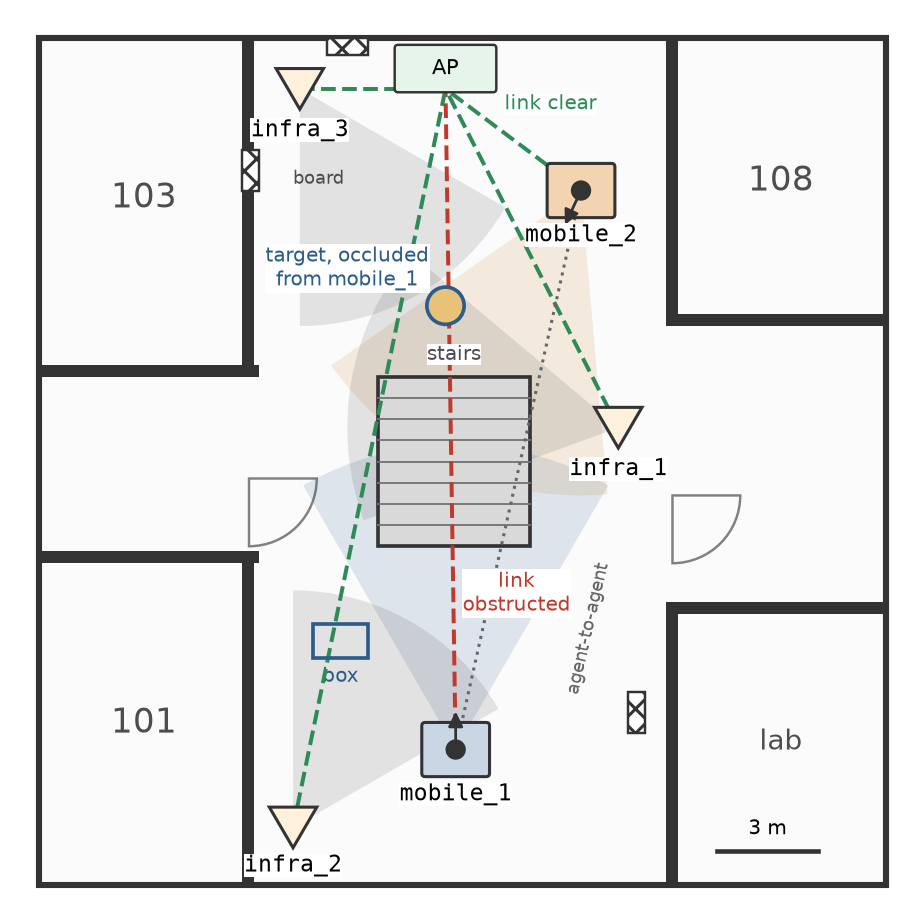
\includegraphics[width=\columnwidth]{figs/fig01_overview.png}
\caption{System overview. Capture, reference and geometry, and
benchmark.}
\label{fig:overview}
\end{figure}


\texttt{mobile\_1} is an AgileX Scout Mini equipped with an Ouster
LiDAR, a ZED~2i stereo camera with an integrated IMU, two IWR6843
mmWave radars, and an RTL8852BU Wi-Fi interface. It also carries
\texttt{sniffer}, a Raspberry Pi~4 whose BCM43455c0 chipset is used
for CSI extraction. \texttt{mobile\_2} is a pushcart equipped with a
RealSense D455 RGB-D camera with IMU, an on-board visual SLAM
pipeline, an IWR6843 radar, and a Wi-Fi interface \todo{confirm
mobile\_2 radar and Wi-Fi part}. Each infrastructure agent,
\texttt{infra\_N}, is a mast with an Arducam RGB camera, an IWR6843
radar, and a Raspberry Pi whose on-board BCM43455 serves as the
wireless interface. The sensor models, rates, and resolutions are
listed in Table~\ref{tab:sensors}.

In each agent, a fixed rig is used to compound multi-modal sensors.
The rig is constant throughout the dataset recording, removing the
need for calibration in every recording session
(Fig.~\ref{fig:platforms}). The sensors of each platform are
expressed in the origin frame of that platform, and each platform is
expressed in the world frame of its site
(Sec.~\ref{sec:groundtruth}). The origin frame depends on the
platform. For \texttt{mobile\_1} we use the robot's
\texttt{base\_link}, so that sensor data and poses are expressed
relative to the body that moves and can be related to wheel odometry
and control. \texttt{mobile\_2} has no robot body, so its LiDAR is
used as the origin, as it provides the strongest metric. For the
infrastructure agents, which carry no LiDAR, the origin is the
camera. The estimation of each transform is described in
Sec.~\ref{sec:calibration}.

\begin{figure}[t]
\centering
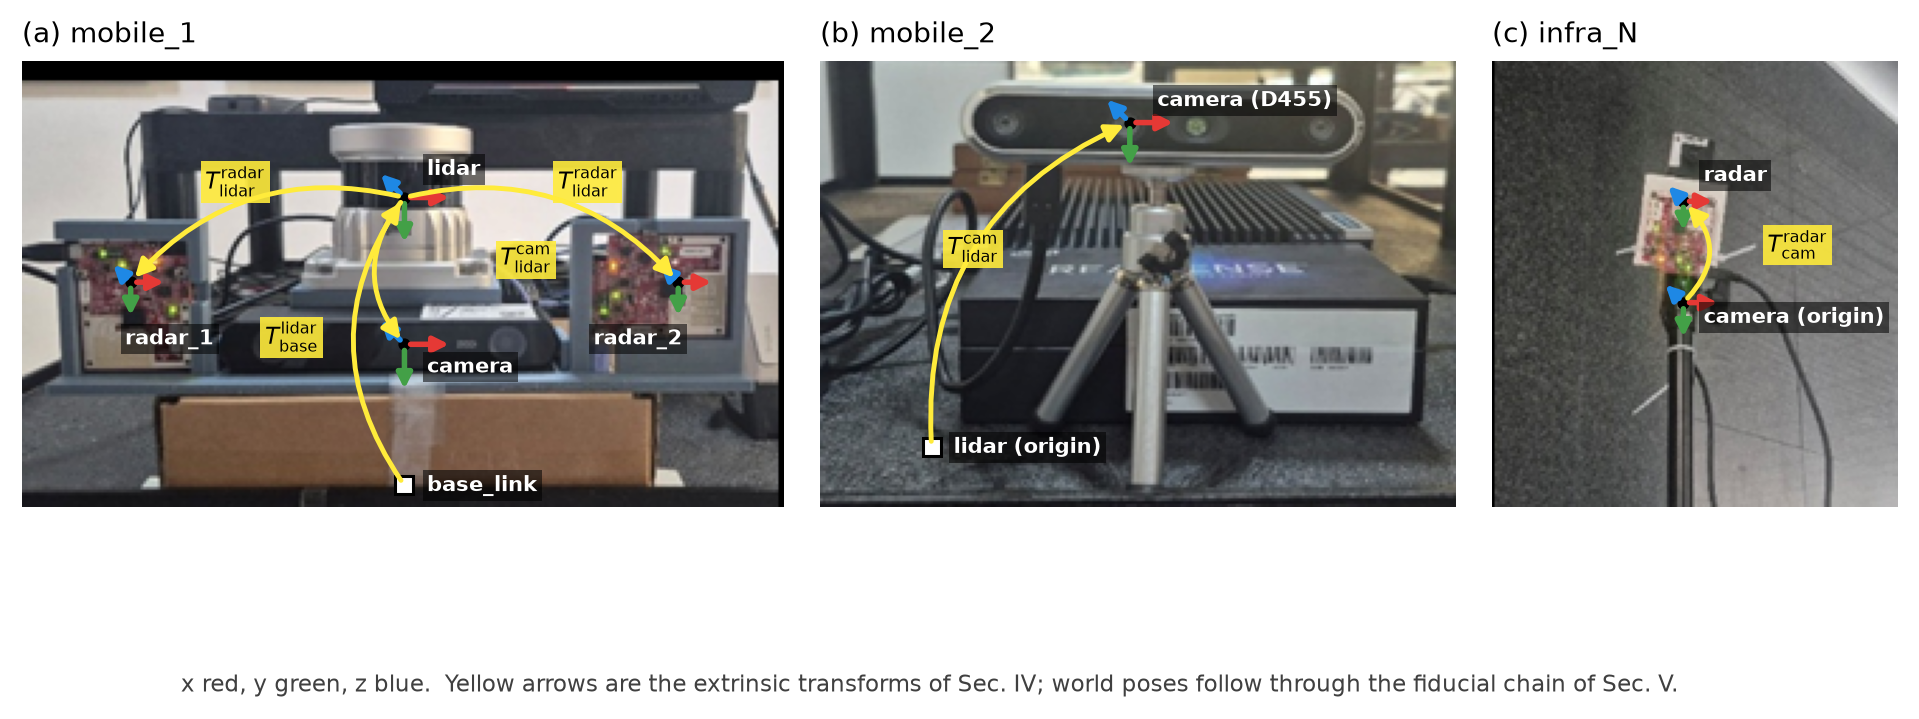
\includegraphics[width=\columnwidth]{figs/fig02_platforms.png}
\caption{Platforms, sensor placement, and the origin frame of each.
\todo{Replace drawn panels with photographs, keeping the frame
arrows.}}
\label{fig:platforms}
\end{figure}


\begin{table*}[!t]
\caption{Per-Agent Sensor Specifications}
\begin{center}
\renewcommand{\arraystretch}{1.2}
\setlength{\tabcolsep}{4pt}
\scriptsize
\begin{tabular}{@{}p{2.0cm} p{2.6cm} p{5.6cm} p{1.9cm} p{2.1cm} p{1.5cm}@{}}
\toprule
\textbf{Equipment} & \textbf{Model Type} & \textbf{Characteristics} & \textbf{Resolution} & \textbf{FoV} & \textbf{Rate} \\
\midrule
\multicolumn{6}{@{}l}{\textit{Mobile Agents}} \\
LiDAR & Ouster OS1-128 & 100 m range & 1024 $\times$ 128 & 45$^\circ$ vert. & 10 Hz \\
LiDAR & Ouster OS0-64 & 50 m range & 1024 $\times$ 64 & 90$^\circ$ vert. & 10 Hz \\
Stereo Camera & ZED 2i & RGB stereo, baseline 120 mm & 1920 $\times$ 1080 & 110$^\circ$ $\times$ 70$^\circ$ & 30 Hz \\
 & & IMU 6-axis, barometer, magnetometer & -- & -- & 400 Hz \\
RGBD & RealSense D455 & RGB, global shutter & 1280 $\times$ 800 & 90$^\circ$ $\times$ 65$^\circ$ & 30 Hz \\
 & & Stereo IR, global shutter, baseline 95 mm & 1280 $\times$ 720 & 87$^\circ$ $\times$ 58$^\circ$ & 30 Hz \\
 & & IMU BMI 055 & -- & -- & 200 Hz \\
 Radar & TI IWR6843ISK & 60--62 GHz, 3 TX / 4 RX & \shortstack[l]{7.5\,cm range \\ $14.2^\circ$ az., $57^\circ$ el.} & $\pm$60$^\circ$ az., $\pm$20$^\circ$ el & 10 Hz \\
Radar & TI IWR6843ISK & 62--64 GHz, 3 TX / 4 RX & \shortstack[l]{7.5\,cm range \\ $13.8^\circ$ az., $55^\circ$ el.} & $\pm$60$^\circ$ az., $\pm$20$^\circ$ el & 10 Hz \\
Radar & TI MMWCAS-RF-EVM & 76--81 GHz, 4$\times$ AWR2243 cascade, 12 TX / 16 RX & \todo{--} & \todo{--} & \todo{--} Hz \\
CSI extractor & RPi 4B (BCM43455c0) & Nexmon, monitor mode, 80 MHz, 1 antenna & 256 subcarriers & -- & $\sim$100 Hz \\
Wi-Fi USB Dongle &  D-Link AX1800 & USB, 5 GHz 802.11ac; iw / iperf3 endpoint & -- & -- & 5/1 Hz \\
Computer &  MIC-713-OX4B2 & NVIDIA Jetson AGX Orin & -- & -- & -- \\

\midrule
\multicolumn{6}{@{}l}{\textit{Infrastructure Agents}} \\
RGB Camera & Arducam B0495 & AR0234, color global shutter, M12 lens & 1920 $\times$ 1200 & 95$^\circ$ diag. & 30 Hz \\
Radar & TI IWR6843ISK & 61.75--64 GHz, 3 TX / 4 RX & \shortstack[l]{7.5\,cm range \\ $13.9^\circ$ az., $56^\circ$ el.} & $\pm$60$^\circ$ az., , $\pm$20$^\circ$ & 10 Hz \\
CSI extractor & RPi 4B (BCM43455c0) & Nexmon, monitor mode, 80 MHz, 1 antenna & 256 subcarriers & -- & $\sim$100 Hz \\
Wi-Fi USB Dongle & Edimax N150 & USB, 5 GHz 802.11ac; iw / iperf3 endpoint & -- & -- &  5/1 Hz \\

\bottomrule
\end{tabular}
\end{center}
\label{tab:sensors}
\end{table*}


Table~\ref{tab:topics} lists the recorded topics per unit. Ouster
data is stored as raw packets together with the sensor's metadata
message, which allows lossless re-decoding through the vendor driver
at any later time \unsure{; the decoded \SI{10}{\hertz} clouds are
included for convenience}. \texttt{mobile\_2} provides an RGB-D
module (color, aligned depth, and both infrared imagers with
\texttt{CameraInfo} and factory extrinsics) and the full output of
its on-board GPU visual SLAM pipeline, including the drifting
visual-odometry path, the loop-closed path, and the tracker status.
This gives a self-contained on-robot estimate that can be compared
against collaborative methods. Infrastructure units provide an RGB
camera and a radar each.

The wireless measurements of Sec.~\ref{sec:commgt} are recorded on
the same timeline as ordinary topics: \texttt{wifi/status}
(\SI{5}{\hertz} passive PHY and reliability state),
\texttt{wifi/iperf} and \texttt{wifi/iperf\_r2r} (active goodput and
RTT), and \texttt{ntp/status} and \texttt{ntp/events} (clock offset,
jitter, and discrete clock events). The CSI stream from
\texttt{sniffer} is recorded in its own bag as raw Nexmon frames; the
devkit parses it into a NumPy/HDF5 representation time-joined to the
reference poses.

\begin{table*}[!t]
\caption{Recorded topics per unit (representative rates).}
\label{tab:topics}
\begin{center}
\renewcommand{\arraystretch}{1.2}
\setlength{\tabcolsep}{4pt}
\scriptsize
\begin{tabular}{@{}p{6.2cm} p{6.6cm} p{2.6cm}@{}}
\toprule
\textbf{Topic (namespace)} & \textbf{Message Type} & \textbf{Rate} \\
\midrule
\multicolumn{3}{@{}l}{\textit{\texttt{mobile\_1/}}} \\
\texttt{ouster/lidar\_packets} & \texttt{ouster\_sensor\_msgs/PacketMsg} & 640 Hz \\
\texttt{ouster/imu\_packets} & \texttt{ouster\_sensor\_msgs/PacketMsg} & 100 Hz \\
\texttt{ouster/metadata} & \texttt{std\_msgs/String} & latched \\
\texttt{radar\{1,2\}/radar/points\_all} & \texttt{PointCloud2} & 10 Hz \\
\texttt{zed/left/image\_rect\_color} & \texttt{Image} (+\,\texttt{CameraInfo}) & 15 Hz \\
\texttt{zed/depth/depth\_registered} & \texttt{Image} & 15 Hz \\
\texttt{zed/imu/data}, \texttt{zed/imu/mag} & \texttt{Imu}, \texttt{MagneticField} & 200 / 50 Hz \\
\texttt{zed/odom}, \texttt{zed/pose}, \texttt{zed/path\_*} & \texttt{Odometry}, \texttt{PoseStamped}, \texttt{Path} & 15 Hz \\
\texttt{tf}, \texttt{tf\_static} & \texttt{TFMessage} & --- \\
\addlinespace
\multicolumn{3}{@{}l}{\textit{\texttt{mobile\_2/}}} \\
\texttt{color/image\_raw} & \texttt{Image} (+\,\texttt{CameraInfo}) & 30 Hz \\
\texttt{depth/image\_rect\_raw} & \texttt{Image} (+\,\texttt{CameraInfo}) & 30 Hz \\
\texttt{infra\{1,2\}/image\_rect\_raw} & \texttt{Image} (+\,\texttt{CameraInfo}) & 30 Hz \\
\texttt{extrinsics/depth\_to\_infra\{1,2\}} & \texttt{realsense2\_camera\_msgs/Extrinsics} & latched \\
\texttt{imu} & \texttt{Imu} & 200 Hz \\
\texttt{visual\_slam/tracking/*}, \texttt{status} & \texttt{Odometry}, \texttt{PoseStamped}, \texttt{Path} & 30 Hz \\
\addlinespace
\multicolumn{3}{@{}l}{\textit{\texttt{infra\_N/}}} \\
\texttt{image\_raw} & \texttt{Image} (+\,\texttt{CameraInfo}) & 30 Hz \\
\texttt{radar/points\_all} & \texttt{PointCloud2} & 10 Hz \\
\addlinespace
\multicolumn{3}{@{}l}{\textit{\texttt{sniffer/}}} \\
\texttt{csi} & \unsure{\texttt{csi\_msgs/Csi}} & $\sim$100--140 Hz \\
\addlinespace
\multicolumn{3}{@{}l}{\textit{All units}} \\
\texttt{wifi/status} & \texttt{wifi\_monitor\_msgs/WifiLinkStatus} & 5 Hz \\
\texttt{wifi/iperf}, \texttt{wifi/iperf\_r2r} & \texttt{wifi\_monitor\_msgs/IperfResult} & per test \\
\texttt{ntp/status}, \texttt{ntp/events} & \texttt{ntp\_monitor\_msgs/NtpStatus}, \texttt{String} & 10 Hz / event \\
\bottomrule
\end{tabular}
\end{center}
\end{table*}


\begin{figure}[t]
\centering
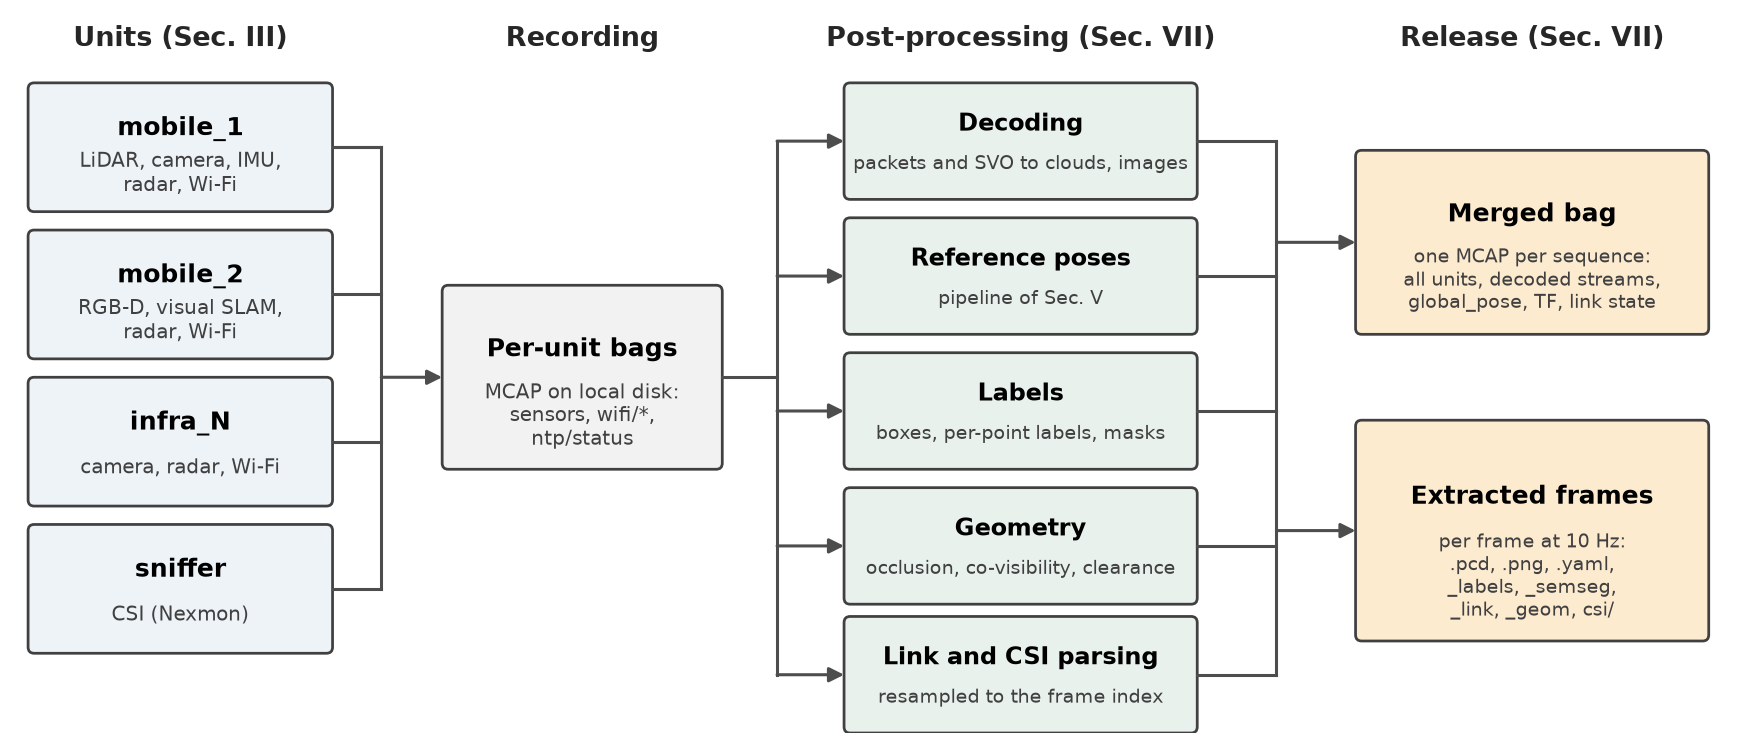
\includegraphics[width=\columnwidth]{figs/fig03_dataflow.png}
\caption{Data flow from sensors to release files.}
\label{fig:dataflow}
\end{figure}


%=======================================================================
\section{Calibration}
\label{sec:calibration}
Two calibrations are required to relate the streams. The spatial
calibration places every sensor in the origin frame of its platform.
The temporal calibration places every measurement on a common
timeline. Each is validated with data that was not used in its
estimation. The placement of platforms in the world frame is part of
the ground truth and is described in Sec.~\ref{sec:groundtruth}.

\subsection{Spatial Calibration}
\label{sec:spatial}
Three transforms are estimated per platform. On \texttt{mobile\_1},
\Ttransform{Base}{LiDAR} is obtained by hand-eye calibration: the
robot is driven through a sequence of motions, and the transform is
solved from the pairs of relative motions reported by wheel odometry
and by LiDAR odometry \bib{hand-eye calibration}. On both mobile
agents, \Ttransform{LiDAR}{Camera} is obtained by direct, target-free
alignment of image and point-cloud features \bib{koide direct
lidar-camera}. For the radar, whose returns are too sparse for
feature alignment, \Ttransform{LiDAR}{Radar} is obtained with a
corner reflector placed at several positions \bib{radar-lidar
calibration} (Fig.~\ref{fig:spatial}).

For the infrastructure rig, the camera and radar are mounted on the
same fixed bracket and calibrated once against a LiDAR by the same
method, which gives \Ttransform{Camera}{Radar} directly. Since the
rig is fixed, the extrinsic remains valid once the sensors are placed
on the infrastructure. The world pose of each infrastructure camera
is obtained during the mapping session through the fiducial chain of
Sec.~\ref{sec:fiducials}.

\begin{figure}[t]
\centering
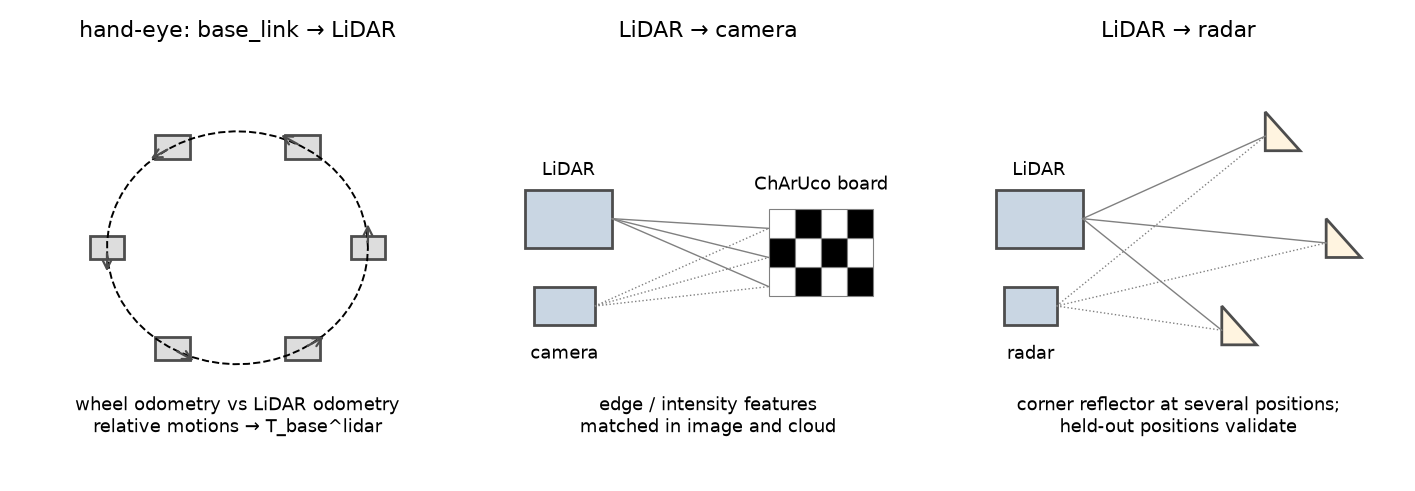
\includegraphics[width=\columnwidth]{figs/fig04_calibration.png}
\caption{Spatial calibration: hand-eye motion sequence for
\Ttransform{Base}{LiDAR}, board features for
\Ttransform{LiDAR}{Camera}, corner reflector for
\Ttransform{LiDAR}{Radar}. \todo{Add residual panel once measured.}}
\label{fig:spatial}
\end{figure}


\subsection{Temporal Calibration}
\label{sec:temporal}
Each unit records its own bag, so frames from different agents are
related only through their timestamps. Two conditions must hold: the
clocks of the units must agree, and each stamp must be close to the
time at which its measurement was taken. We address each condition
below and then bound the remaining error.

\subsubsection{Clock Synchronization}
The clocks are synchronized with chrony. \texttt{mobile\_1} acts as
the server, and every other agent and \texttt{sniffer} act as clients
polling every \SI{8}{\second}. This traffic passes over the measured
link, but at a few hundred bytes per poll it is negligible, and since
it is present in every run it forms part of the channel that the
benchmark replays. Recording starts only after every unit reports a
converged offset. Each unit logs its offset and any clock adjustment
(\texttt{ntp/status}, \texttt{ntp/events}) into its own bag, so the
alignment at any frame can be checked and poorly aligned frames can
be filtered out.

Table~\ref{tab:ntp} and Fig.~\ref{fig:clock} summarize the result
over \unsure{1} sequences. No clock was stepped during any recording,
and the worst pairwise offset is \unsure{about
\SI{70}{\micro\second}}.

\begin{table}[t]
\centering
\caption{Clock synchronization across all sequences (server:
\texttt{mobile\_1}). RMS offset per sequence, summarized as median and
maximum over sequences.
\unsure{Values from a single live pass; update once all sequences are processed.}}
\label{tab:ntp}
\footnotesize
\begin{tabular}{@{}lccccc@{}}
\toprule
& \multicolumn{2}{c}{RMS offset} & & & \\
\cmidrule(lr){2-3}
Client & Median & Max & Jitter (med.) & Path delay (med.) & Steps \\
\midrule
\texttt{mobile\_2} & \SI{10.9}{\micro\second} & \SI{10.9}{\micro\second} & \SI{227}{\micro\second} & \SI{4.2}{\milli\second}  & 0 \\
\texttt{infra\_1}  & \SI{42.5}{\micro\second} & \SI{42.5}{\micro\second} & \SI{175}{\micro\second} & \SI{4.1}{\milli\second}  & 0 \\
\texttt{sniffer}   & \SI{28.7}{\micro\second} & \SI{28.7}{\micro\second} & \SI{619}{\micro\second} & \SI{15.6}{\milli\second} & 0 \\
\bottomrule
\end{tabular}
\end{table}


\begin{figure}[t]
\centering
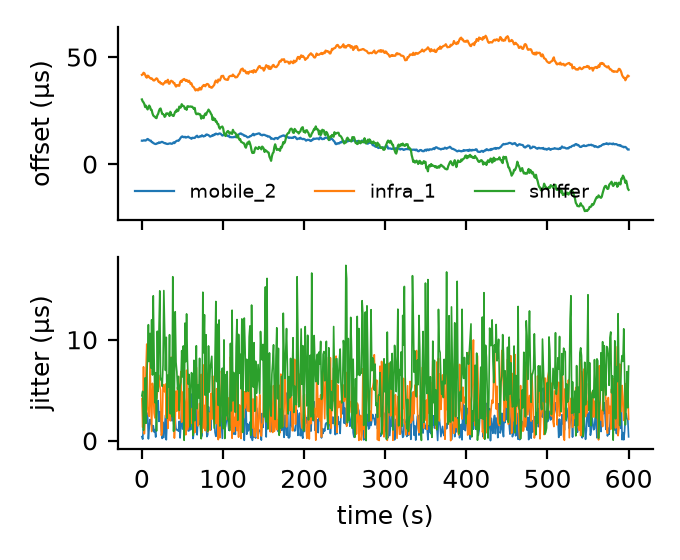
\includegraphics[width=\columnwidth]{figs/fig05_clock.png}
\caption{Clock offset (top) and jitter (bottom) of each client against
\texttt{mobile\_1} over one session. \todo{Replace dummy data.}}
\label{fig:clock}
\end{figure}


These offsets describe the stability of each clock relative to the
server, not its accuracy. NTP assumes a symmetric path delay, and any
asymmetry appears as a constant bias that chrony cannot observe. This
is relevant only for \texttt{sniffer}, which reaches the server over
its \SI{2.4}{\giga\hertz} management link with a path delay several
times larger than that of the other units, so its bias may be as
large as half that delay, \SI{7.8}{\milli\second}. We measure the
bias directly from the probe packets that \texttt{mobile\_2} sends
and \texttt{sniffer} captures. Each packet is stamped at transmission
on the clock of \texttt{mobile\_2} and at reception on the clock of
\texttt{sniffer}. Since the packet is in flight for only nanoseconds,
the difference between the two stamps equals the bias of the sniffer
plus its driver latency. The median difference over a run is
\todo{}, which bounds the bias.

\subsubsection{Timestamp Latency}
Agreeing clocks are not sufficient if the stamps themselves are
late. Every message is stamped on arrival at its host, so each stamp
lags its measurement by the transport latency of that sensor
\todo{estimates per sensor: LiDAR over Ethernet, cameras over USB,
radar over UART}, and camera stamps lag further by the exposure time.
These lags are approximately constant for a given sensor. We leave
the stamps as recorded so that users can apply their own correction,
for example by aligning the motion observed by each sensor.

\subsubsection{Motion Compensation and Fusion Error Bounds}
\label{sec:temporal_bounds}
Both conditions reduce to a timing error $\Delta t$, which displaces
a measurement taken on a platform moving at speed $v$ by
\begin{equation}
  \delta x = v \, \Delta t .
  \label{eq:time_bound}
\end{equation}
We take $v_{\max} = \SI{3}{\metre\per\second}$ as an upper bound on
agent speed. The clock offset of \unsure{\SI{70}{\micro\second}} then
corresponds to \unsure{\SI{0.2}{\milli\metre}}, and the sniffer bias
of \todo{} to \todo{}, which is \todo{}\,\% of the half-wavelength
$\lambda/2 = \SI{26.1}{\milli\metre}$ at \SI{5745}{\mega\hertz} that
sets the CSI sampling requirement. Transport latency and exposure are
larger: a constant lag of \SI{10}{\milli\second} corresponds to
\SI{3}{\centi\metre}, but since it is constant it can be estimated
and removed. The largest term is the LiDAR sweep, which takes
\SI{100}{\milli\second} at \SI{10}{\hertz}, so the first and last
points of a scan can be \SI{30}{\centi\metre} apart. This is removed
by per-point deskewing with IMU-propagated motion in the reference
pipeline \cite{glim}.

Combining the terms that remain after compensation, the worst-case
intra-frame spatial error at $v_{\max}$ is
\begin{equation}
  \delta x_{\max} = v_{\max}\,\big(\Delta t_{\mathrm{clk}}
  + \Delta t_{\mathrm{lat}} + \Delta t_{\mathrm{exp}}\big)
  = \todo{Y}\,\si{\centi\metre},
  \label{eq:fusion_bound}
\end{equation}
where $\Delta t_{\mathrm{clk}}$ is the worst clock offset,
$\Delta t_{\mathrm{lat}}$ the largest uncorrected transport latency,
and $\Delta t_{\mathrm{exp}}$ the longest camera exposure. The LiDAR
sweep is excluded because it is deskewed.

The error budget is therefore dominated by sensor physics and
transport, not by synchronization. Clock alignment contributes well
under a millimetre, while the larger terms are either compensated,
as for the LiDAR sweep, or constant and removable, as for per-sensor
latency.

\subsection{Calibration Validation}
\label{sec:calib_val}
Each extrinsic is checked on data that was not used in its
estimation. For \Ttransform{LiDAR}{Camera}, the LiDAR returns on the
ChArUco boards of the mapping session are projected into the image
and compared with the detected board corners; the reprojection
residual is reported per board and per range. For
\Ttransform{LiDAR}{Radar}, the corner reflector is placed at
positions not used in calibration, and the radar detection is
compared with the LiDAR centroid of the reflector. For
\Ttransform{Base}{LiDAR}, the hand-eye result is checked through the
board residual of Sec.~\ref{sec:gt_val}: a board observed from
\texttt{mobile\_1} predicts a board pose through
\Ttransform{Base}{LiDAR} and \Ttransform{LiDAR}{Camera}, so the
residual tests both transforms at once and is not reported
separately. For the infrastructure rig, \Ttransform{Camera}{Radar} is
checked in the same way as the mobile radar, with the rig mounted in
place. Table~\ref{tab:calib} lists the residuals per sensor pair. The
same values are stored in the release
(\texttt{calibration/residuals.json}) so that users can weight each
transform according to its accuracy.

\begin{table}[t]
\centering
\caption{Calibration residuals on held-out observations.}
\label{tab:calib}
\footnotesize
\setlength{\tabcolsep}{4pt}
\begin{tabular}{@{}llll@{}}
\toprule
Transform & Check & Median & p95 \\
\midrule
\Ttransform{LiDAR}{Camera}  & board corner reprojection (px) & \todo{} & \todo{} \\
\Ttransform{LiDAR}{Radar}   & reflector offset (cm)          & \todo{} & \todo{} \\
\Ttransform{Base}{LiDAR}    & board pose via chain (cm, deg) & \todo{} & \todo{} \\
\Ttransform{Camera}{Radar}  & reflector offset (cm), infra   & \todo{} & \todo{} \\
Clock, all clients          & offset to \texttt{mobile\_1} (\si{\micro\second}) & \todo{} & \todo{} \\
Clock, \texttt{sniffer}     & probe-packet bias (ms)         & \todo{} & \todo{} \\
\bottomrule
\end{tabular}
\end{table}


%=======================================================================
\section{Ground Truth}
\label{sec:groundtruth}
Our reference combines three of the strategies reviewed in
Sec.~\ref{sec:related}. The reference map is SLAM-derived, which
removes the survey scanner normally required for map registration.
Every scan is registered against this map, so the pose is carried by
the map and not by odometry between anchors. Fiducial boards, posed
in the map frame during the mapping session, anchor the RGB-D agent
and the infrastructure where registration alone is weak. Since the
annotations and the collaboration geometry are both derived from
these poses, the reference is built and validated to annotation
grade and not only as an evaluation target. The link is recorded on
the same timeline and is the fourth reference that the benchmark
replays (Sec.~\ref{sec:commgt}).

\subsection{Reference Poses and Map}
\label{sec:gt}
The reference map is built in a dedicated mapping session and held
fixed afterwards; no dataset sequence contributes to it. A second,
separate mapping pass is recorded and processed independently and is
used only to cross-check the first. A LiDAR-inertial SLAM solution
\cite{glim} estimates the mapping trajectory, with sub-mapping and
loop closure tuned for offline accuracy and checked so that no submap
is left without a long-range constraint. The map is then frozen and
every scan is re-registered into it by point-to-plane ICP against
local plane fits, iterated until the pose corrections fall below the
sensor noise. This follows the prior-map registration used by the
survey-grade datasets \cite{newercollege,oxfordspires,lamar}, with
the prior built by our own sensors instead of a survey scanner. Plane
fits are used instead of nearest-neighbour targets for a specific
reason: within a surface smeared by accumulated drift, a
\SI{3.0}{\centi\metre} scan offset produces only
\SI{0.5}{\centi\metre} of nearest-neighbour residual, so the error
would not be visible to conventional ICP.

This frozen map is the metric backbone of the sequences. The
LiDAR-equipped agents are localized by scan-to-map registration, and
the RGB-D agent, \texttt{mobile\_2}, by registering its depth point
cloud against the same map. All trajectories therefore share one
metric frame by construction and do not require post-hoc alignment.
Inter-agent relative poses reduce to two registration errors against
shared local geometry instead of two accumulated drifts, and since no
dataset sequence contributes to the map, the agreement of each agent
with the map is an out-of-sample check.

\begin{figure}[t]
\centering
\fbox{\parbox[c][5cm][c]{0.95\columnwidth}{\centering
\todo{Fig.~6: reference map of one site with the fiducial network.
Boards used for initialisation and drift bounding in one colour,
held-out validation boards in another; AP and infrastructure poses
marked.}}}
\caption{Reference map with the fiducial network and held-out boards.}
\label{fig:refmap}
\end{figure}


\subsection{Fiducial Network}
\label{sec:fiducials}
The reference map provides the shared metric frame, but a
sensor-constrained agent cannot enter it by registration alone. A
cold-start ICP against a building-scale map may converge in a wrong
basin, and between registrations the visual odometry of the agent
accumulates drift, fastest in feature-poor regions where the local
geometry only weakly constrains the alignment. We therefore deploy a
network of printed ChArUco boards in the environment. The boards are
not surveyed independently: the pose of each board is estimated in
the reference frame from the observations of the mapping session
itself, so the network inherits the metric accuracy of the map. This
is sparse anchoring as in \cite{airmuseum}, with the anchors posed by
the map instead of by survey equipment.

During the mapping session, the mapping agent, which carries a LiDAR
and a camera, loops around the site and stops at each board to
record several views of it. With the mapping trajectory
\Ttransform{World}{LiDAR} from Sec.~\ref{sec:gt} and the extrinsic
\Ttransform{LiDAR}{MobileCamera} from Sec.~\ref{sec:spatial}, the
pose of each board is
\begin{equation}
   \Ttransform{World}{Board} = \Ttransform{World}{LiDAR} \times \Ttransform{LiDAR}{MobileCamera} \times \Ttransform{MobileCamera}{Board} .
   \label{eq:board_chain}
\end{equation}
One board serves as the origin of the world frame,
\Ttransform{World}{OriginBoard}, and every mobile agent starts at a
board, so that each run begins at a known pose.

Infrastructure agents are placed in the same frame through the
boards. During the mapping session, a
\(500\,\mathrm{cm} \times 500\,\mathrm{cm}\) ChArUco board is shown to
the mobile and infrastructure cameras in the same frame. Each camera
computes its pose relative to the board,
\Ttransform{Board}{MobileCamera} and \Ttransform{Board}{InfraCamera},
and the world pose of the infrastructure camera is
\begin{equation}
\begin{split}
  \Ttransform{World}{InfraCamera} = {}
    & \Ttransform{World}{LiDAR} \times \Ttransform{LiDAR}{MobileCamera} \times \\
    &  (\Ttransform{Board}{MobileCamera})^{-1} \times \Ttransform{Board}{InfraCamera} .
\end{split}
\label{eq:infra_camera_chain}
\end{equation}

The boards serve three roles. At the start of a sequence, a board
sighting provides the absolute initial pose that places the first
registration in the correct convergence basin. Along the trajectory,
board sightings provide absolute pose observations that bound the
drift accumulated by visual odometry between map registrations; for
this reason the boards are placed mainly in feature-poor regions,
where both visual tracking and depth registration are weakest.
Finally, the boards are used to validate the registration of every
subsequent sequence, as described in Sec.~\ref{sec:gt_val}.

\subsection{Validation}
\label{sec:gt_val}
Convergence of the refinement in Sec.~\ref{sec:gt} establishes
self-consistency, not accuracy. The plane targets are themselves
estimated from the map, so a self-consistent deformation would
converge equally well. Accuracy is therefore established by three
checks that did not enter the estimation. They are summarized in
Table~\ref{tab:gt} and Fig.~\ref{fig:gt_errors} along two axes: where
the surfaces are, and how consistently the poses place them.

\paragraph{Second mapping pass.} Surfaces are measured by their
thickness, defined as the p95--p5 spread of points about planes
fitted to \SI{0.25}{\metre} patches, and always compared with the
sensor noise floor obtained from individual sweeps, which carry no
pose error. After refinement, floor surfaces are within
\SI{1}{\centi\metre} of that floor, while walls, observed at longer
range and shallower incidence, remain above it. The larger wall
thickness of Sequence B comes from extended single-visit corridor
sections, where no revisit constrains the lateral placement; floors,
observed at short range throughout, are unaffected. The second
recording, captured four weeks later and processed independently,
reproduces the surface placement to \SI{1.06}{\centi\metre} on walls,
with the relative scale agreeing to $2\times10^{-5}$. This agreement
establishes the scale \emph{stability} between sessions that share a
sensor. Since both runs share the sensor and the algorithm, a
deformation common to both would not be visible in this test.

\paragraph{Control distances.} The absolute scale is established by
laser-rangefinder control distances measured between marked points on
walls and pillars at the scale of the site, \todo{$N$ distances of
\SIrange{5}{40}{\metre} per site}. Their disagreement with the map
grows with the scale at which a common deformation would act, which
closes the gap left by the second pass. \todo{Report per site: mean
and max map-minus-rangefinder error.}

\paragraph{Held-out boards.} The pose of each board in the map is
fixed by the mapping session. When an agent sights a board during a
sequence, its registered pose and camera extrinsic predict where the
board should appear, and the difference between this prediction and
the observed board pose is a residual that did not enter the
registration. It is therefore an independent check at that frame.
For the RGB-D agent, whose trajectory uses board sightings as
constraints, a subset of boards is held out of the estimation and the
residual is evaluated on those boards only. \todo{Report the median
and 95th-percentile board residual, in translation and rotation, per
agent.}

\paragraph{Pose consistency.} Per-scan consistency is measured where
the same surface is observed twice: by the same robot minutes apart,
and by different robots on overlapping routes. The second case tests
the full chain of each robot (registration, extrinsic calibration,
and time association) at LiDAR accuracy for the LiDAR pair, and
isolates the sensor-constrained mechanism for the RGB-D robot.

\paragraph{Interpretation.} The two axes have different error
budgets. A smooth deformation displaces surfaces without thickening
them, since the scans remain locally consistent, so the residual
thickness is per-scan placement scatter, which averages out in the
map. The cross-session comparison bounds the disagreement between
the surface placement of two runs, here about one centimetre, and
the control distances bound what both runs could have in common.
Annotations are placed against the fused map and therefore inherit
centimetre-level geometry; per-scan placement scatter and pose-level
fusion are governed by the repeat-visit, cross-robot, and board
figures. We release the reference as a validated pseudo-ground truth
on these terms: it is established from onboard sensing alone, and the
independent measurements are used only to check the result, never to
produce it.

\begin{table}[!t]
\centering
\caption{Pseudo Ground Truth Map Quality}
\label{tab:gt}
\begin{tabular}{llc}
\toprule
& Quantity & Value \\
\midrule
\multicolumn{3}{l}{\emph{Surface geometry}} \\
\quad Thickness, seq.\ A & walls / floors & 7.4 / 2.6 cm \\
\quad Thickness, seq.\ B & walls / floors & -- \\
\quad Sensor noise floor & walls / floors & 2.7 / 1.4 cm \\
\quad Cross-session      & surface placement, walls & -- \\
\quad Cross-session      & relative scale & -- \\
\quad Control distances  & rangefinder, median & -- \\
\midrule
\multicolumn{3}{l}{\emph{Pose consistency}} \\
\quad Refinement         & final pose correction & 0.23 cm, 0.022$^\circ$ \\
\quad Repeat-visit       & same robot, 2-scan walls & 2.9 cm \\
\quad Cross-robot        & LiDAR vs.\ LiDAR & -- \\
\quad Cross-robot        & LiDAR vs.\ RGB-D & -- \\
\bottomrule
\end{tabular}
\end{table}


\begin{figure}[t]
\centering
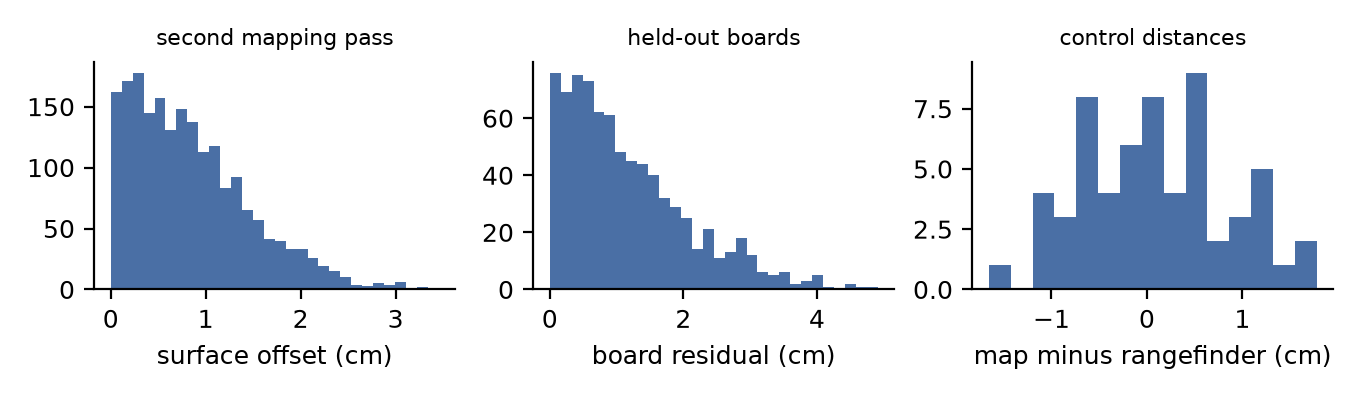
\includegraphics[width=\columnwidth]{figs/fig07_gt_errors.png}
\caption{Ground-truth error distributions from the three independent
checks. \todo{Replace dummy data.}}
\label{fig:gt_errors}
\end{figure}


\subsection{Perception Annotations}
\label{sec:annotations}
Static objects are annotated once, as 3D boxes in the map frame, and
projected into the frames of every agent through the reference
poses. One annotation therefore yields a label in every frame in
which the object appears, with the same position, size, and identity
across agents, as required for collaborative fusion, and it places
each object in the map from which occlusion and visibility are
ray-cast (Sec.~\ref{sec:paradigms}). Since the labels are projected
through the poses, a pose error becomes a label error. Each projected
box is therefore checked against the sensor returns it encloses, so
that a pose error appears as a detectable misfit. \todo{Report the
fraction of frames whose projected boxes enclose their object's
returns, and the threshold used.}

Dynamic objects cannot be placed once in the map and are annotated
per timestep in the world frame. At each timestep, the registered
point clouds of all agents are fused in the map frame, and the
points explained by the static map are removed, leaving only the
points that moved. The remaining points are clustered, each cluster
is fitted with a box, and the boxes are linked across time into a
track, so that one object keeps one identity across timesteps and
across agents. Annotators verify and correct these proposals on
keyframes at \todo{rate}, and the boxes are interpolated between
keyframes. Since the boxes are in the world frame, they are projected
into the frames of every agent through the reference poses in the
same way as static boxes, and the same occlusion, visibility, and
evidence quantities are computed for them (Sec.~\ref{sec:paradigms}).

Because boxes and the reference map share one frame, two further
labels follow without additional annotation. Every LiDAR or depth
point inside a box inherits the class of the box, which gives a 3D
semantic label per point for every agent and frame. This also holds
for dynamic objects, whose points are already separated from the
background by the static-map subtraction and inherit the class of
their per-timestep box. Likewise, a class assigned once to each
surface of the reference map (floor, wall, furniture) is inherited by
every registered frame at that site. Dense image masks for static
content are obtained by rendering the labelled map from each
reference pose, with occlusion handled by the renderer; their
accuracy is bounded by the reference, so the box-fit check above is
reported with them. A dynamic object is absent from the map mesh, so
its mask cannot be rendered. For these objects we project the in-box
points into the image, which gives a sparse mask, and add hand-drawn
masks on keyframes, interpolated between them. \todo{State what is
released: boxes, per-point labels, rendered masks for static objects
and surfaces, projected and keyframe masks for dynamic objects.
Annotation tool, QA process, and class statistics per class and per
environment; add a statistics figure.}

\begin{figure}[t]
\centering
\fbox{\parbox[c][4.5cm][c]{0.95\columnwidth}{\centering
\todo{Fig.~8: annotation examples. One frame from two agents: 3D
boxes on the LiDAR scan, per-point labels, rendered mask on the
image, with the same object identity across agents.}}}
\caption{Annotation examples: boxes, per-point labels, and rendered
masks.}
\label{fig:annotations}
\end{figure}


\subsection{Communication Ground Truth}
\label{sec:commgt}
The link is recorded on the same timeline as the sensing streams at
two levels: the link state, which describes what the network
delivered, and the channel state, which describes the propagation
that produced it. Both are replayed by the benchmark of
Sec.~\ref{sec:benchmarks}: a message sent at time $t$ over link
$(a,b)$ is delayed, truncated, or dropped according to the goodput,
RTT, and loss measured on that link at $t$, so the cost of the link
is measured against the link the agents actually had.
Fig.~\ref{fig:linktrace} shows one sequence.

All agents associate to a single access point on channel 149 (VHT-80,
\SI{5745}{\mega\hertz}); no ad hoc or mesh mode is used. Two
transmitter settings are imposed by the CSI receiver, which is a
1$\times$1 802.11ac part. 802.11ax is disabled, since the receiver
cannot demodulate HE frames and would capture only control frames,
and the number of spatial streams is fixed to one, since a
single-antenna receiver cannot separate a two-stream transmission.
The second setting also suits the geometric predictors of
Sec.~\ref{sec:paradigms}, since two-stream capacity depends on the
scattering richness, which map-derived geometry does not capture.
Power save is disabled on all transmitters. The measured
single-stream capacity is \numrange{275}{282}\,Mbit/s uplink and
\numrange{598}{676}\,Mbit/s downlink per mobile agent.

\emph{Link state.} Passive metrics are read at \SI{5}{\hertz} from
the kernel wireless interface: RSSI, negotiated bitrate and MCS,
transmit retries and failures, and channel busy ratio. During
outages the monitor continues publishing with
\texttt{associated=false}, so coverage gaps appear as explicit
labels and not as missing samples. Active metrics are obtained with
\texttt{iperf3} \cite{iperf3} in \SI{4}{\second} tests, uplink and
downlink separately. Different configurations are set up in each
pass. In survey mode, each agent owns the whole channel. In
cooperation mode, several agents run their tests at the same time by
design, so the measured goodput includes the contention that a
deployed team would face when agents share the channel, and the
traces replayed by the benchmark carry that contention with them.
Latency is measured as ICMP round-trip time at \SI{100}{\hertz}:
\SI{3.3}{\milli\second} when idle and
\SIrange{60}{109}{\milli\second} under load, the latter caused by
queueing and not by path loss.

\emph{Channel state.} CSI is extracted with Nexmon \cite{nexmon} on
a BCM43455c0 in monitor mode at \SI{80}{\mega\hertz}, which yields
one estimate over 242 used subcarriers per received frame from its
VHT-LTF. The extractor, \texttt{sniffer}, is a separate host carried
on \texttt{mobile\_1}, with a \SI{2.4}{\giga\hertz} management link
kept off the measured band; it captures the frames of
\texttt{mobile\_2} and \texttt{infra\_1}. Only QoS data frames give
full-bandwidth estimates. Control frames are captured, since they are
useful for diagnosing PHY problems, but they are excluded from the
analysis, since mixing them changes the effective bandwidth from
frame to frame. The achieved data-frame rates were \SI{141}{\hertz}
from \texttt{infra\_1} and \SI{104}{\hertz} from \texttt{mobile\_2}.

The channel varies over roughly half a wavelength of motion,
$\lambda/2 = \SI{26.1}{\milli\metre}$ at \SI{5745}{\mega\hertz}. If
three estimates per half-wavelength are required to follow these
variations, the achieved rates are sufficient up to a relative speed
of about \SI{1.2}{\metre\per\second}; above that, the CSI is too
sparse to resolve them. The rate cannot simply be raised by sending
more packets, since Wi-Fi aggregates many packets into one
transmission and each transmission yields a single channel estimate
from its preamble. Disabling aggregation would raise the CSI rate but
would also distort the throughput being measured. CSI phase is not
coherent across devices, which run on independent oscillators, so
each transmitter--receiver pair is treated as an independent sensing
link.

\begin{figure}[t]
\centering
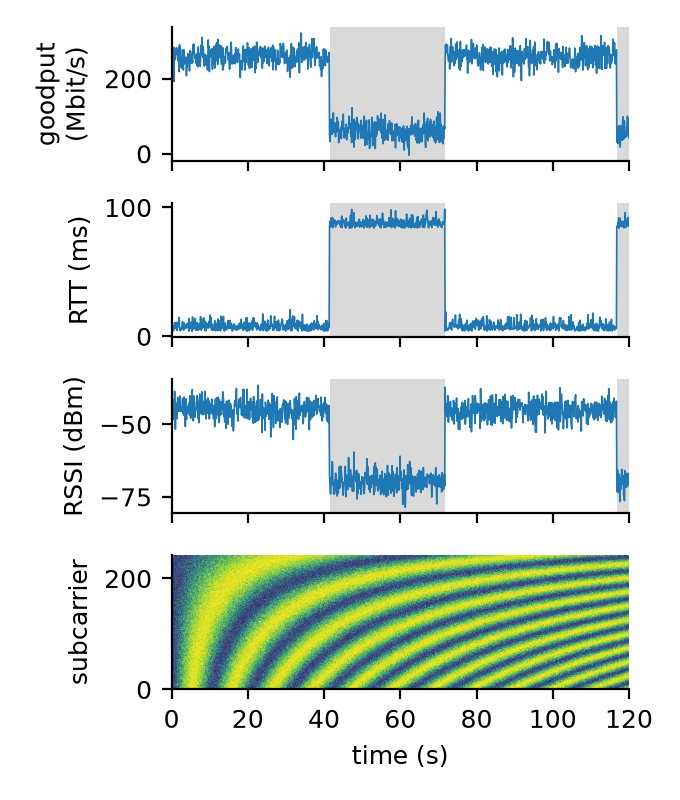
\includegraphics[width=\columnwidth]{figs/fig09_link_trace.png}
\caption{Link trace over one sequence: goodput, RTT, RSSI, and CSI
amplitude. Shaded spans are frames with $\mathrm{clear}(a,b) < 0.6$.
\todo{Replace dummy data.}}
\label{fig:linktrace}
\end{figure}


%=======================================================================
\section{Dataset Design and Collection}
\label{sec:collection}

\subsection{Environments}
\label{sec:environments}
Data collection was conducted at three indoor sites on the Guangfu
Campus of National Yang Ming Chiao Tung University (NYCU)
(Fig.~\ref{fig:sites}). Site selection was governed by three factors,
each associated with a quantity the release reports per frame rather
than with a qualitative descriptor.

\textit{Viewpoint}: the availability of an elevated, persistent
vantage and its attainable lateral displacement from the mobile
agents, characterized by the range of aspect angles $\beta$ between an
ego and a helper. \textit{Appearance}: illumination, texture, and
clutter density, which determine the range beyond which
$\mathrm{visible}(i)$ ceases to imply $\mathrm{observed}(i)$
(Eqs.~\eqref{eq:visible}--\eqref{eq:observed}). \textit{Radio
propagation}: whether structure intervenes between an agent and the
access point, characterized by first-Fresnel-zone clearance.

Prior sensing-and-communication datasets infer blockage from received
power \cite{deepsense6g}; we compute clearance geometrically and
validate it against measured RSSI (Sec.~\ref{sec:results}), so that
link state is an independent label rather than a threshold on the
signal it explains. Each site is mapped once as a dense point cloud
(Sec.~\ref{sec:gt}), with all agent poses expressed in a single
anchored map frame, so that occlusion, co-visibility, and link
geometry are evaluated against a common geometric representation.
The three sites differ in layout, corridor width, wall material, and
access point placement. This spread in map geometry is what makes the
held-out site of Sec.~\ref{sec:q2} a test of transfer to a new
building and not an interpolation within one.

\begin{figure}[t]
\centering
\fbox{\parbox[c][4cm][c]{0.95\columnwidth}{\centering
\todo{Fig.~10: three sites. Map cloud, infrastructure pose, AP
position, and both mobile trajectories, one panel per site.}}}
\caption{The three sites with access point and infrastructure
positions.}
\label{fig:sites}
\end{figure}


\subsection{Collection Protocol}
\label{sec:protocol}
Recordings are organised at three levels. A \emph{site} is one floor
with its own reference map and fiducial network. A \emph{session} is
one visit to a site; the map is frozen at the start of the session
and the reference is validated against the held-out boards at its
end, and sessions differ in the conditions listed in
Sec.~\ref{sec:conditions}. A \emph{sequence} is one recording within
a session with one paradigm assignment and one channel-load mode.
Sequence identifiers carry all three levels
(\texttt{site1/session02/seq05}), which shows directly which
sequences share a map and which share conditions. Every site
contains the full paradigm table (Table~\ref{tab:paradigms}) in at
least \todo{two} sessions, so that the same geometry is observed
under different link conditions and a model trained on two sites has
seen every paradigm several times.

One mobile agent is designated the \textit{ego} and is viewpoint
limited by design, either by trajectory as it gets routed in
structures that intervene between it and the annotated objects or by
sensing budget, carrying the shorter-range depth sensor. The second
mobile agent is the \textit{partner}. Ego assignment alternates across
runs, so that a reported condition is attributable to the geometry
rather than to a platform.

Infrastructure agents are never assigned the ego role, their function
being the elevated, persistent vantage that no mobile node can
sustain. Existing multi-robot and roadside datasets collaborate
between sensors at a common height \cite{s3e,inscope} so the elevation
asymmetry is absent by construction, and assigning the infrastructure
node as ego would reinstate that symmetry.

\begin{figure*}[t]
\centering
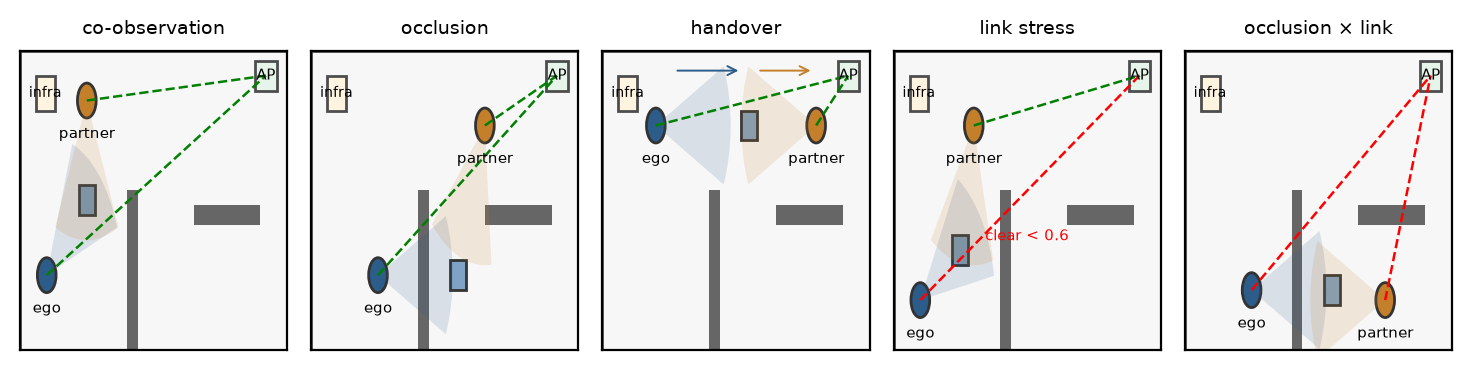
\includegraphics[width=\textwidth]{figs/fig11_paradigms.png}
\caption{Paradigms illustrated on one site. Ego in blue, partner in
orange, annotated object in the box, fields of view shaded; green
dashed links are clear, red are obstructed ($\mathrm{clear} < 0.6$).}
\label{fig:paradigms_fig}
\end{figure*}


\subsubsection{Collaboration Geometry Characterization}
\label{sec:paradigms}

\begin{table*}[t]
\centering
\caption{Per-sequence descriptors}
\label{tab:seq}
\footnotesize
\setlength{\tabcolsep}{3pt}
\resizebox{\textwidth}{!}{%
\begin{tabular}{@{}lllll ccc cccc ccc@{}}
\toprule
\multicolumn{5}{c}{Design} & \multicolumn{3}{c}{Geometry} &
\multicolumn{4}{c}{Complementary observations} & \multicolumn{2}{c}{Link, scene} \\
\cmidrule(r){1-5}\cmidrule(lr){6-8}\cmidrule(lr){9-12}\cmidrule(l){13-14}
Sequence & Site & Paradigm & Stressor & Ego &
$C$ & $\beta_{\textsf{inf}}$ & $\beta_{\textsf{pr}}$ & \textsf{Ep.} &
\textsf{Occ} & \textsf{Ev} RGB-D & \textsf{Ev} LiDAR & Dopp. &
NLoS (\%) & Obj. \\
\midrule
\multirow{2}{*}{\texttt{coop2\_0828}} & \multirow{2}{*}{MIRC} &
\multirow{2}{*}{co-observation} & \multirow{2}{*}{none} &
\texttt{m1}$^\ast$ & 0.5 & 149/0.67 & 146/0.74 & 9 (3\textsf{i},2\textsf{p})
& 0.10 & 0.29 & 0.01 & --- & 33 & 2 \\
 & & & & \texttt{m2} & 0.5 & 29/0.33 & 145/0.83 & 8 (1\textsf{i},2\textsf{p})
& 0.02 & 0.39 & --- & --- & 18 & 2 \\
\bottomrule
\end{tabular}}
\end{table*}


The quantities defined here serve two purposes. They characterise the
condition under which each frame was recorded, so that results can be
stratified by it; and they are the predictor set $\mathcal{G}$ of
Sec.~\ref{sec:q2}, used to test how much of the link's cost could
be foreseen from the map alone. Both purposes require them to be
computed per frame from the map, the annotations, and the agent poses,
never from the signal they are meant to predict. A paradigm specifies
a trajectory geometry together with the condition that geometry is
intended to induce. Each paradigm is a predicate over per-frame
quantities, computed from the map, the annotations, and the node
poses, and released with the recordings rather than asserted of a run.

Consider one annotated object at one frame. Let $e$ denote the ego and
$j$ range over the remaining nodes. For node $i$, let
$\omega_i \in [0,1]$ be the fraction of rays cast from $i$'s sensor
origin to the object surface that are blocked by mapped structure,
$r_i$ the range to the object, and $n_i$ the evidence returns falling
within the annotated box such as LiDAR points, depth points, or
projected pixel area, according to the node's primary modality. With
$\tau = 0.5$,
%
\begin{align}
\mathrm{visible}(i) &\equiv \text{in FoV} \;\wedge\; \omega_i < \tau,
\label{eq:visible}\\
\mathrm{observed}(i) &\equiv \mathrm{visible}(i) \;\wedge\; n_i \ge n_{\min,i}
\;\wedge\; r_i \le r_{\max,i}.
\label{eq:observed}
\end{align}
%
Visibility is geometric, requiring only an unobstructed line, while
observation is evidential: the sensor returned support sufficient for
a detection, within the range at which that modality still returns
anything. Both have single-agent precedent (Sec.~\ref{sec:related});
here they are computed for every node and kept distinct, so that an
object the ego could not see remains separable from one it could see
but for which it returned too little evidence, a separation that
carries the analysis of Sec.~\ref{sec:findings}. A node $j \ne e$ is
a \emph{helper} if $\mathrm{visible}(j)$, and the best helper
$j^\star$ is that of lowest $\omega$; the aspect angle $\beta$
subtended at the object between the rays to $e$ and to $j^\star$
distinguishes a redundant viewpoint near $0^\circ$ from a
complementary one beyond $90^\circ$. Each frame further carries the
co-visibility fraction $C$, objects visible to at least two nodes over
those visible to at least one.

Per link, state is computed geometrically rather than from received
power. A direct-ray test over-reports clear links, since an obstacle
near the path diffracts energy out of it; the first Fresnel zone, of
radius $r_1 = \sqrt{\lambda d_1 d_2 / d}$, bounds the region where
such obstruction matters, and a link is conventionally treated as
free-space when at least $0.6\,r_1$ is clear \cite{itup530}. At
\SI{5.75}{\giga\hertz} this radius is \SI{28}{\centi\metre} at the
midpoint of a \SI{6}{\metre} link, so indoors the criterion
distinguishes furniture beside the path from furniture on it. We
therefore report $\mathrm{clear}(a,b)$, the minimum clearance along
the link normalised by $r_1$, with $\mathrm{clear}(a,b) < 0.6$ the
obstructed criterion, and validate it against measured RSSI in
Sec.~\ref{sec:results}. Fig.~\ref{fig:geometry} shows these
quantities over one sequence.

\begin{figure}[t]
\centering
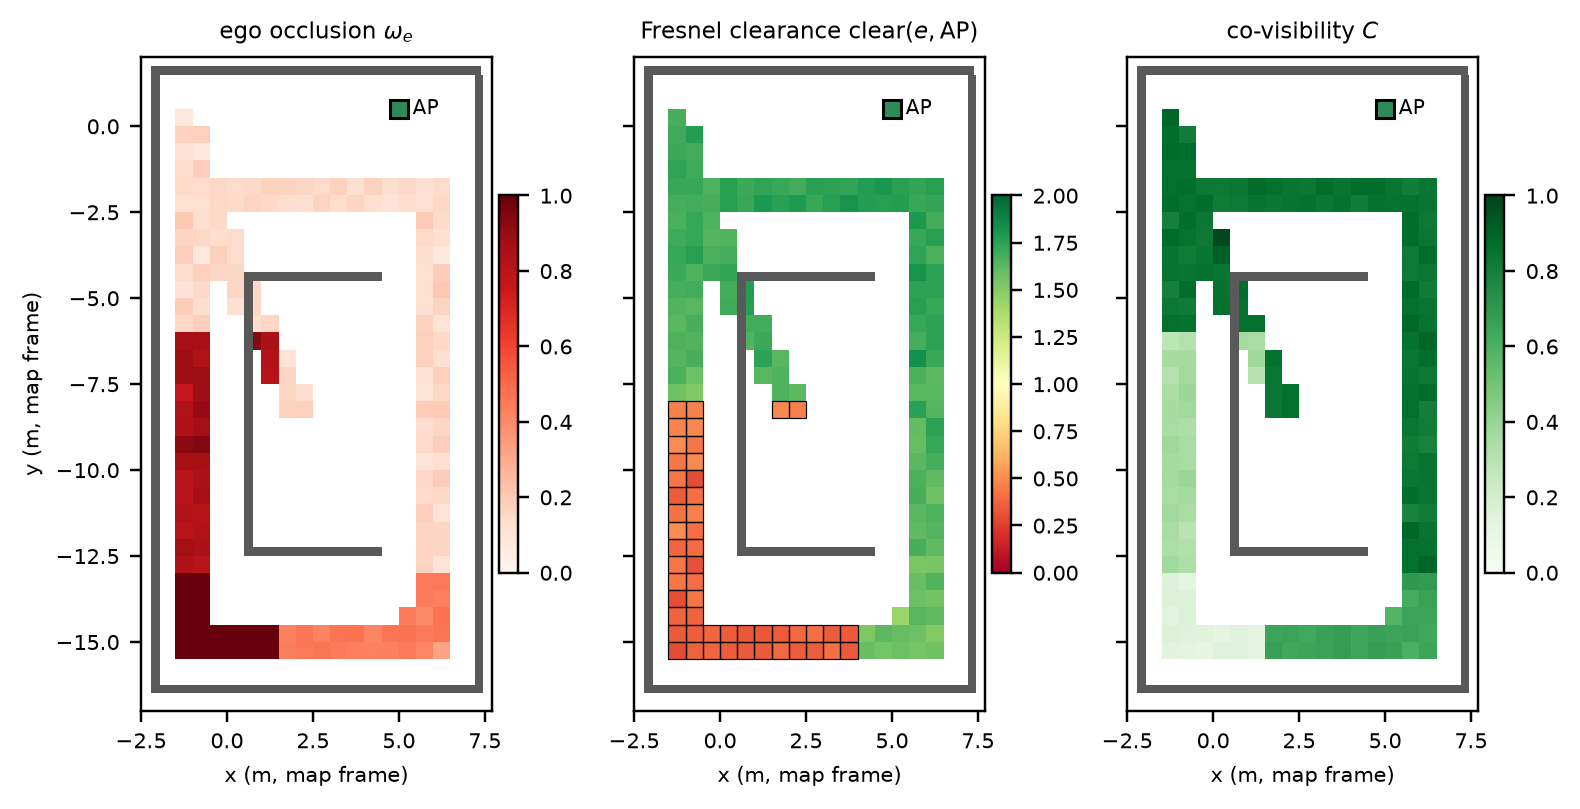
\includegraphics[width=\columnwidth]{figs/fig12_geometry.png}
\caption{Per-frame geometry over one sequence: ego occlusion
$\omega_e$, Fresnel clearance to the best helper with the 0.6
threshold, and co-visibility $C$. \todo{Replace dummy data.}}
\label{fig:geometry}
\end{figure}


Table~\ref{tab:paradigms} composes these into the paradigms, evaluated
in order so that a condition combining occlusion with a degraded link
is reported as such rather than absorbed into the plain occlusion
class.

\begin{table}[t]
\centering
\caption{Trajectory Paradigms Evaluation}
\label{tab:paradigms}
\footnotesize
\setlength{\tabcolsep}{4pt}
\begin{tabular}{@{}cll@{}}
\toprule
\# & Paradigm & Condition \\
\midrule
1 & Co-observation     & $\mathrm{visible}(e) \;\wedge\; \text{helper}$ \\
2 & Occlusion          & $\neg\,\mathrm{visible}(e) \;\wedge\; \text{helper}$ \\
3 & Handover          & $\lvert \{ i : \mathrm{visible}(i) \} \rvert = 1$ \\
4 & Link stress             & $\text{helper} \;\wedge\; \mathrm{clear}(e,j^\star) < 0.6$ \\
5 & Occlusion $\times$ link & $\neg\,\mathrm{visible}(e) \;\wedge\; \text{helper} \;\wedge\; \mathrm{clear}(e,j^\star) < 0.6$ \\
6 & Unstructured       & none of the above \\
\bottomrule
\end{tabular}
\end{table}


A label is assigned per frame from the measured quantities, not
declared once for a run: a sequence intended as co-observation carries
occlusion labels wherever the geometry produced them. Results are
therefore stratified by the underlying quantities ($\omega$, $\beta$,
$r$, $C$, and clearance), not by the paradigm label, which discards
their magnitude and depends on the chosen thresholds; the label
describes a frame's condition, while the quantities are what
evaluation is conditioned on.

\begin{table}[t]
\centering
\caption{Pipeline parameters, frozen across sequences.}
\label{tab:params}
\footnotesize
\setlength{\tabcolsep}{4pt}
\begin{tabularx}{\columnwidth}{@{}l>{\raggedright\arraybackslash}X@{}}
\toprule
Parameter & Value \\
\midrule
\multicolumn{2}{@{}l}{\emph{Occlusion}}\\
\quad occupancy voxel      & \SI{10}{\centi\metre} \\
\quad rays per object      & 200 per agent and frame \\
\addlinespace
\multicolumn{2}{@{}l}{\emph{Evidence floors}}\\
\quad LiDAR                & 1 point \\
\quad depth                & 50 points \\
\quad camera               & \SI{400}{px^2} \\
\addlinespace
\multicolumn{2}{@{}l}{\emph{Range caps}}\\
\quad Ouster, infra        & \SI{20}{\metre} \\
\quad ZED                  & \SI{4.5}{\metre} \\
\quad RealSense            & \SI{5}{\metre} \\
\addlinespace
\multicolumn{2}{@{}l}{\emph{Link}}\\
\quad centre frequency     & \SI{5.775}{\giga\hertz} ($\lambda = \SI{5.19}{\centi\metre}$) \\
\addlinespace
\multicolumn{2}{@{}l}{\emph{Workarounds}}\\
\quad outlier removal      & 20 neighbours, $2\sigma$ \\
\quad sensor self-clearance & \SI{0.6}{\metre} \\
\quad link endpoint clearance & \SI{0.7}{\metre} \\
\bottomrule
\end{tabularx}
\end{table}


Table~\ref{tab:params} lists the pipeline parameters, frozen across
sequences. Range caps are set from the range at which median in-box
evidence falls to its floor, then fixed. Three parameters are
workarounds rather than modeling choices. Outlier removal deletes
isolated points from the registered map, which would otherwise appear
as floating obstacles and block rays spuriously. The self and
endpoint clearances exist because the sensors, the infrastructure
mast, and the access point are themselves part of the mapped
structure, so every ray would otherwise be blocked where it starts;
the cost is that obstacles within these distances of an endpoint are
not detected.

\subsection{Conditions Captured}
\label{sec:conditions}
Geometry varies across sites, and conditions vary across sessions.
Each site is recorded in several sessions that repeat the same
paradigm assignments under different occupancy, illumination,
furniture placement, and channel load, so that the same map geometry
is observed under different link conditions. This repetition allows
Sec.~\ref{sec:q2} to separate the part of the link cost that the map
explains from the part that the conditions add.
Table~\ref{tab:sessions} lists, per session, the site, the date and
time of day, the occupancy (people per minute crossing the ego path,
counted from the annotations), the interference (channel busy ratio
at idle), the channel load mode, and any furniture changes since the
mapping session. \todo{Fill Table~\ref{tab:sessions} and report
totals: sessions, sequences, hours, distance, frames, annotated
instances, per site.}

\begin{table}[t]
\centering
\caption{Sessions and their conditions.}
\label{tab:sessions}
\footnotesize
\setlength{\tabcolsep}{3pt}
\begin{tabular}{@{}lllllll@{}}
\toprule
Session & Site & Time & Occupancy & Busy & Load & Seq. \\
\midrule
\texttt{s1/01} & 1 & \todo{} & \todo{} & \todo{} & survey & \todo{} \\
\texttt{s1/02} & 1 & \todo{} & \todo{} & \todo{} & coop.  & \todo{} \\
\texttt{s2/01} & 2 & \todo{} & \todo{} & \todo{} & survey & \todo{} \\
\texttt{s2/02} & 2 & \todo{} & \todo{} & \todo{} & coop.  & \todo{} \\
\texttt{s3/01} & 3 & \todo{} & \todo{} & \todo{} & survey & \todo{} \\
\texttt{s3/02} & 3 & \todo{} & \todo{} & \todo{} & coop.  & \todo{} \\
\bottomrule
\end{tabular}
\end{table}


\begin{figure}[t]
\centering
\fbox{\parbox[c][3.5cm][c]{0.95\columnwidth}{\centering
\todo{Fig.~13: session conditions. Occupancy and channel busy ratio
per session, grouped by site.}}}
\caption{Occupancy and interference across sessions.}
\label{fig:sessions}
\end{figure}


%=======================================================================
\section{Data Format, Structure, and Development Kit}
\label{sec:format}

\subsection{Release Formats}
The dataset ships in two formats generated from the same recordings.
The \emph{raw format} preserves the original ROS~2 bags at native
rates with original timestamps and QoS, replayable into a live ROS
graph; this is required for SLAM, odometry, and latency-sensitive
work, where arrival order and link timing are part of the problem. The
\emph{extracted format} reorganizes the same data into per-frame files
in an OPV2V-style layout~\cite{opv2v}, so existing collaborative
detection codebases can consume it unmodified. Every extracted frame
records its source bag, topic, and original message timestamp, so
results trace back to the raw stream.

Raw sequences are ROS~2 bags (rosbag2, MCAP, uncompressed), split at
\SI{2}{GiB}, each with a \texttt{metadata.yaml} giving per-topic
counts, QoS, and per-chunk timing, so sequences can be indexed without
opening the MCAP files. MCAP embeds the message definitions, so bags
can be read without the recording workspace. Each unit records
locally: no sensor stream traverses the wireless network before
reaching disk, since the link is a measured quantity rather than a
transport. Messages retain their arrival stamps on the unit's own
clock (Sec.~\ref{sec:temporal}); in parallel each unit logs its offset
and jitter against \texttt{mobile\_1} (\texttt{ntp/status},
\SI{10}{\hertz}) and discrete clock events (\texttt{ntp/events}). The
devkit maps any stamp onto the common timebase, so users may work with
raw per-unit timestamps or the corrected timeline, and may filter by
the alignment quality prevailing at capture.

\subsection{Release Structure}
The raw release follows the site, session, and sequence hierarchy of
Sec.~\ref{sec:protocol}. The reference map, boards, and control
distances are stored once per site, since every session of a site
shares them (Fig.~\ref{fig:release}).

{\scriptsize
\begin{verbatim}
dataset/
|- metadata/            # index, sensor specs
|- calibration/         # intrinsics, extrinsics,
|                       #   residuals.json
|- site_X/
|  |- reference/        # reference map, surface labels,
|  |                    #   boards, control distances
|  `- session_YY/
|     |- metadata.json  # conditions (Table VI)
|     `- seq_ZZ/
|        |- metadata.json     # units, intended_paradigm
|        |- units/{mobile_*,infra_*,sniffer}/   # *.mcap
|        |- csi/ comms/ sync/ # channel, link, clock logs
|        |- geometry/         # per-frame collaboration
|        |                    #   geometry (Sec. VI)
|        `- annotations/ poses/   # boxes, per-point labels,
|                                 #   masks; reference poses
`- devkit/
\end{verbatim}
}

The extracted release mirrors this per frame at a fixed
\SI{10}{\hertz}: split, sequence, unit, then one file group per
synchronized frame keyed by a zero-padded index, with \texttt{.pcd}
clouds, \texttt{.png} images, and a \texttt{.yaml} carrying the
unit's pose, calibration, and annotated objects. The first unit in a
sequence's \texttt{metadata.yaml} is the ego, matching the convention
fusion codebases expect; any mobile unit may be re-designated as ego
through the devkit.

{\scriptsize
\begin{verbatim}
extracted/<split>/site_X_session_YY_seq_ZZ/
|- metadata.yaml        # ego, units, conditions
|- mobile_1/
|  |- 000001.pcd            # lidar
|  |- 000001_radar1.pcd     # radar
|  |- 000001_radar2.pcd     # radar
|  |- 000001_cam0.png       # cameras
|  |- 000001.yaml           # pose (map frame),
|  |                        #  calib, boxes
|  |- 000001_link.yaml      # RSSI, MCS, retries,
|  |                        #  goodput, RTT, clock offset
|  |- 000001_geom.yaml      # per object: omega, visible,
|  |                        #  observed, r, n; per link:
|  |                        #  clearance; paradigm label
|  |- 000001_labels.npy     # class per point of 000001.pcd
|  `- 000001_semseg.png     # rendered semantic mask (static),
|                           #  projected/keyframe mask (dynamic)
|- mobile_2/ infra_1/ ...
`- csi/                 # per-frame CSI tensors
\end{verbatim}
}

Three per-frame files have no counterpart in existing collaborative
perception datasets. \texttt{\_link.yaml} attaches each unit's
wireless state at that instant, with its clock offset, so that
bandwidth-, latency-, and asynchrony-conditioned fusion can be trained
and evaluated directly from the frame index. \texttt{\_geom.yaml}
attaches the collaboration geometry of Sec.~\ref{sec:paradigms}
computed for that unit, so results can be stratified by it and the
predictors of Sec.~\ref{sec:q2} read without rerunning the pipeline.
\texttt{csi/} holds the corresponding channel-state tensors on the
same keys. \texttt{\_labels.npy} and \texttt{\_semseg.png} carry the
per-point and per-pixel labels of Sec.~\ref{sec:annotations}; the
mask's provenance (rendered, projected, or keyframe) is recorded per
object in \texttt{.yaml}, so users can filter by it. Extraction is
deterministic and scripted, so users may regenerate it at other frame
rates, sensor subsets, or synchronization tolerances.

\begin{figure*}[t]
\centering
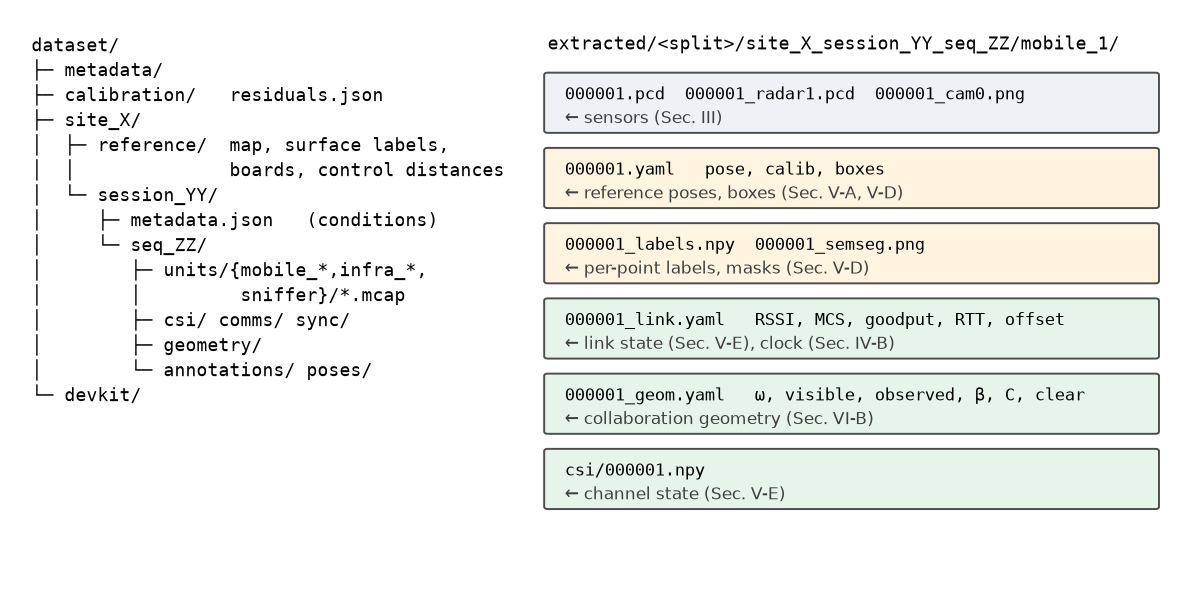
\includegraphics[width=\textwidth]{figs/fig14_release.png}
\caption{Release tree and the files of one extracted frame, each
pointing to the section that defines it.}
\label{fig:release}
\end{figure*}


\subsection{Development Kit}
\label{sec:devkit}
The benchmark of Sec.~\ref{sec:benchmarks} can be reproduced from the
devkit alone; no code outside the release is required. The devkit is
a Python package with six parts.

\begin{enumerate}
\item \emph{Readers.} MCAP readers that do not require a ROS
installation, and loaders for the extracted format that return
synchronized multi-unit samples and time-joined (pose, link, CSI,
geometry) tuples.
\item \emph{Calibration and clock API.} Resolution of any
sensor-to-sensor or sensor-to-world transform at a query time,
including the board-derived infrastructure poses and the residuals of
Table~\ref{tab:calib}; clock utilities that map any stamp onto the
common timebase and export per-frame offset labels.
\item \emph{Projection.} Projection of reference poses, boxes,
per-point labels, and masks into the frame of any unit, with the
in-box evidence check of Sec.~\ref{sec:annotations}; the ego may be
re-designated to any mobile unit.
\item \emph{Geometry.} The per-frame computation of
Sec.~\ref{sec:paradigms} ($\omega$, visible, observed, $\beta$, $C$,
clearance, paradigm label) from the map, annotations, and poses, with
the parameters of Table~\ref{tab:params} exposed so that users can
regenerate \texttt{\_geom.yaml} under other thresholds.
\item \emph{Channel replay.} The module that applies the ideal,
synthetic, and logged channels of Sec.~\ref{sec:channels} to any
message stream, reading goodput, RTT, and link state from
\texttt{\_link.yaml}; the CSI parsers that produce the NumPy/HDF5
representation.
\item \emph{Evaluation.} Fixed splits and scripts for T1 (ATE, RPE,
loop closures, time to merge, merged-map label accuracy) and T2 (AP
at IoU 0.3, 0.5, 0.7; mIoU), the Q1 link-cost and retained-gain
metrics, and the Q2 regression with leave-one-site-out, feature sets,
and the anticipated-share metric. Splits are defined by sequence,
never by frame, to prevent temporal leakage, and by site for Q2.
\end{enumerate}

\subsection{License and Access}
The dataset is released under \todo{license} with a persistent DOI
(\todo{}); the devkit separately under \todo{MIT/Apache-2.0} at
\todo{URL}. All color and infrared streams are anonymized before
release: faces are detected with \todo{detector}, blurred, and
manually reviewed frame by frame for sequences containing bystanders;
unblurred originals are not distributed. Communication identifiers
(BSSIDs, MAC and IP addresses, ESSIDs) are consistently pseudonymized
across the release, so link topology remains analyzable without
exposing the deployment network.

%=======================================================================
\section{Benchmark}
\label{sec:benchmarks}
The benchmark is a single controlled experiment. Two collaborative
tasks are run on the same frames three times, and each time the
inter-agent messages are delivered through a different channel, so
that any difference in accuracy is caused by the channel alone.
Comparing the runs measures the cost of the real link (Q1). Relating
that cost, frame by frame, to the geometry of Sec.~\ref{sec:paradigms}
measures how much of it could have been foreseen from the map (Q2).

\subsection{Channels}
\label{sec:channels}
Under the \emph{ideal} channel, messages arrive complete, in order,
and with zero delay. Under the \emph{synthetic} channel, the
bandwidth is a fixed budget and the delay is drawn from a fixed
distribution, as in prior collaborative perception benchmarks
\cite{where2comm,v2xvit}. Under the \emph{logged} channel, a message
of size $s$ sent at time $t$ over link $(a,b)$ arrives after
$\mathrm{RTT}_{ab}(t)/2 + s/G_{ab}(t)$, where $G_{ab}(t)$ is the
goodput measured on that link at $t$ (Sec.~\ref{sec:commgt}), and it
is dropped if the link was down. One replay module applies all three
channels (Fig.~\ref{fig:replay}), so the channel is the only
variable between runs. Evaluation uses leave-one-site-out over the
three sites (Sec.~\ref{sec:q2}), so that nothing fitted on one site
is evaluated on it. \todo{Sequences and frames per site.}

\begin{figure}[t]
\centering
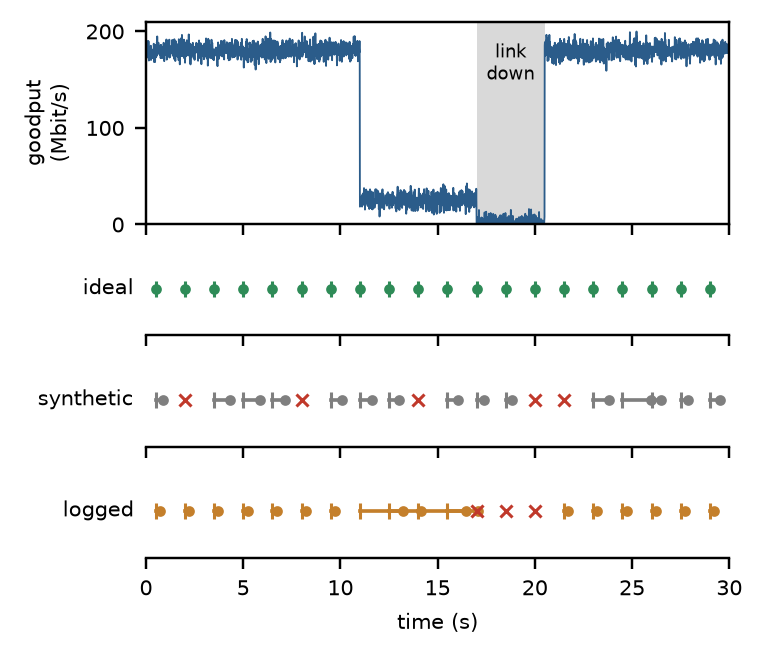
\includegraphics[width=\columnwidth]{figs/fig15_channel_replay.png}
\caption{Channel replay on one sequence. Top: logged goodput $G_{ab}(t)$.
Rows: the same partner messages through the ideal, synthetic, and logged
channels (tick: sent; dot: delivered; cross: dropped). Only the logged
channel reproduces the correlated delays and outages of the real link.}
\label{fig:replay}
\end{figure}


\subsection{Tasks and Baselines}
\label{sec:tasks}
The two tasks correspond to the two processes through which a team
cooperates, and they use the link differently. Collaborative SLAM
exchanges compact descriptors and occasional map fragments, while
collaborative perception exchanges perception data at every frame.
Each task is reported together with a single-agent reference computed
with all messages withheld, since the cooperative result is
meaningful only relative to it. Outdoor-origin methods are
re-parameterised for indoor ranges and object sizes.
\todo{Re-parameterisation table.}

\emph{Collaborative SLAM (T1).} The agents exchange place-recognition
descriptors, loop-closure candidates, and map fragments over the
channel, and produce all trajectories and a merged map in a common
frame. Accuracy is measured as ATE and RPE against the reference
(Sec.~\ref{sec:gt}), with the number of accepted inter-agent loop
closures and the time to the first successful merge as secondary
measures. The baselines are chosen to cover both primary sensors, the
three ways in which a team can use the link, and whether semantic
content is transmitted (Table~\ref{tab:t1}). Swarm-SLAM
\cite{swarmslam} is the primary baseline. It supports LiDAR and RGB-D
front ends, so every agent runs the same system, and it is the system
that the planetary-analogue study gated with logged traces
\cite{planetary_cslam}, which makes our results comparable to the one
prior measured-link C-SLAM study. DiSCo-SLAM \cite{discoslam} is a
second LiDAR system that exchanges continuously instead of at
rendezvous. Since it accepts LiDAR only, it runs on the two
LiDAR-equipped agents, which also shows what a heterogeneous team
loses when a C-SLAM system cannot use every agent's sensor. COVINS-G
\cite{covinsg} is centralised and streams keyframes from every agent
to a server; this places the most traffic on the link and is the
closest to a deployment through an access point. Kimera-Multi
\cite{kimeramulti} labels each agent's map locally and shares only
geometry, so in addition to ATE and RPE it is scored by the label
accuracy of the merged map against the per-point labels of
Sec.~\ref{sec:annotations}. Since no labels cross the link, this
number measures the effect of the link on alignment alone.
Hydra-Multi \cite{hydramulti} streams labelled mesh and scene-graph
fragments to a server, so its label accuracy measures the effect of
the link on the semantic content itself. Compared with Kimera-Multi
it separates the two effects, and compared with COVINS-G it shows
whether a centralised semantic stream costs more than a centralised
geometric one. The single-agent reference is the odometry of each
agent with loop closure and no exchange: GLIM \cite{glim} on the
LiDAR agents, the on-board visual SLAM stream on \texttt{mobile\_2},
and single-robot Kimera for the semantic rows.

\begin{table}[t]
\centering
\caption{T1 baselines.}
\label{tab:t1}
\footnotesize
\setlength{\tabcolsep}{3pt}
\resizebox{\columnwidth}{!}{%
\begin{tabular}{@{}llll@{}}
\toprule
Baseline & Sensor & Exchange & Map \\
\midrule
Swarm-SLAM   & LiDAR, RGB-D  & Rendezvous  & Geometric \\
DiSCo-SLAM   & LiDAR         & Continuous  & Geometric \\
COVINS-G     & Stereo        & Centralised & Geometric \\
Kimera-Multi & Stereo, RGB-D & Continuous  & Semantic, local labels \\
Hydra-Multi  & Stereo, RGB-D & Centralised & Semantic, exchanged \\
\bottomrule
\end{tabular}}
\end{table}


\emph{Collaborative perception (T2).} The ego receives the messages
of its partners and describes the scene in its own frame, either as
3D boxes scored by AP at IoU 0.3, 0.5, and 0.7, or as per-point
semantic labels scored by mIoU. Indoor objects are small, so a few
centimetres of pose error caused by the link can move a box past the
stricter thresholds while it still marks the correct object.
Reporting all three thresholds separates missed objects from
misplaced ones. For detection, the baselines span the range of
message sizes, since the message size is what the link acts on. Early
fusion transmits raw point clouds, the largest message. Late fusion
transmits boxes, the smallest. Where2comm \cite{where2comm} transmits
selected features under a bandwidth budget, which under the logged
channel is set from the measured goodput at each frame. V2X-ViT
\cite{v2xvit} transmits full feature maps with learned latency
compensation, which tests whether compensation tuned on synthetic
delay holds under measured delay. All four share one backbone
\todo{PointPillars}, re-parameterised for indoor ranges and object
sizes. For segmentation, early and late fusion are run on a
point-labelling backbone \todo{Cylinder3D or SPVCNN}, transmitting
raw points and labelled points respectively. Partner messages are
placed in the ego frame using either the reference poses or the T1
estimate; the second option carries the effect of the link on
localization through to perception.

\subsection{Results: What the Link Costs}
\label{sec:results}
For a task with accuracy $A$, the cooperative gain is
$G = A_{\mathrm{ideal}} - A_{\mathrm{ego}}$ and the cost of the link
is $\Delta = A_{\mathrm{ideal}} - A_{\mathrm{logged}}$. We report
$\Delta$ and the retained gain $1 - \Delta/G$ per task and, for T2,
per output (AP for boxes, mIoU for labels)
(Tables~\ref{tab:res_t1}, \ref{tab:res_t2}; Fig.~\ref{fig:q1}). The
synthetic run answers a related question: by how much the impairment
models of prior benchmarks misstate that cost.

\begin{table*}[t]
\centering
\caption{T1 results under the three channels. ATE in cm, RPE in
\%/deg per \SI{10}{\metre}, label accuracy in \% for the semantic
rows.}
\label{tab:res_t1}
\footnotesize
\setlength{\tabcolsep}{4pt}
\begin{tabular}{@{}l cc cc cc cc cc c c@{}}
\toprule
& \multicolumn{2}{c}{Single-agent} & \multicolumn{2}{c}{Ideal} & \multicolumn{2}{c}{Synthetic} & \multicolumn{2}{c}{Logged} & \multicolumn{2}{c}{Label acc.} & $\Delta$ & $1-\Delta/G$ \\
\cmidrule(lr){2-3}\cmidrule(lr){4-5}\cmidrule(lr){6-7}\cmidrule(lr){8-9}\cmidrule(lr){10-11}
Baseline & ATE & RPE & ATE & RPE & ATE & RPE & ATE & RPE & ideal & logged & (ATE) & \\
\midrule
Swarm-SLAM   & \todo{} & \todo{} & \todo{} & \todo{} & \todo{} & \todo{} & \todo{} & \todo{} & -- & -- & \todo{} & \todo{} \\
DiSCo-SLAM   & \todo{} & \todo{} & \todo{} & \todo{} & \todo{} & \todo{} & \todo{} & \todo{} & -- & -- & \todo{} & \todo{} \\
COVINS-G     & \todo{} & \todo{} & \todo{} & \todo{} & \todo{} & \todo{} & \todo{} & \todo{} & -- & -- & \todo{} & \todo{} \\
Kimera-Multi & \todo{} & \todo{} & \todo{} & \todo{} & \todo{} & \todo{} & \todo{} & \todo{} & \todo{} & \todo{} & \todo{} & \todo{} \\
Hydra-Multi  & \todo{} & \todo{} & \todo{} & \todo{} & \todo{} & \todo{} & \todo{} & \todo{} & \todo{} & \todo{} & \todo{} & \todo{} \\
\bottomrule
\end{tabular}
\end{table*}


\begin{table*}[t]
\centering
\caption{T2 results under the three channels, partner data placed by
reference poses. AP in \% at IoU 0.3/0.5/0.7 for detection, mIoU in
\% for segmentation. $\Delta$ and $1-\Delta/G$ at IoU 0.5 and on
mIoU.}
\label{tab:res_t2}
\footnotesize
\setlength{\tabcolsep}{4pt}
\begin{tabular}{@{}ll cccc cc@{}}
\toprule
Output & Baseline & Single-agent & Ideal & Synthetic & Logged & $\Delta$ & $1-\Delta/G$ \\
\midrule
Boxes  & early fusion  & \todo{}/\todo{}/\todo{} & \todo{}/\todo{}/\todo{} & \todo{}/\todo{}/\todo{} & \todo{}/\todo{}/\todo{} & \todo{} & \todo{} \\
Boxes  & late fusion   & \todo{}/\todo{}/\todo{} & \todo{}/\todo{}/\todo{} & \todo{}/\todo{}/\todo{} & \todo{}/\todo{}/\todo{} & \todo{} & \todo{} \\
Boxes  & Where2comm    & \todo{}/\todo{}/\todo{} & \todo{}/\todo{}/\todo{} & \todo{}/\todo{}/\todo{} & \todo{}/\todo{}/\todo{} & \todo{} & \todo{} \\
Boxes  & V2X-ViT       & \todo{}/\todo{}/\todo{} & \todo{}/\todo{}/\todo{} & \todo{}/\todo{}/\todo{} & \todo{}/\todo{}/\todo{} & \todo{} & \todo{} \\
Labels & early fusion  & \todo{} & \todo{} & \todo{} & \todo{} & \todo{} & \todo{} \\
Labels & late fusion   & \todo{} & \todo{} & \todo{} & \todo{} & \todo{} & \todo{} \\
\bottomrule
\end{tabular}
\end{table*}


\begin{figure*}[t]
\centering
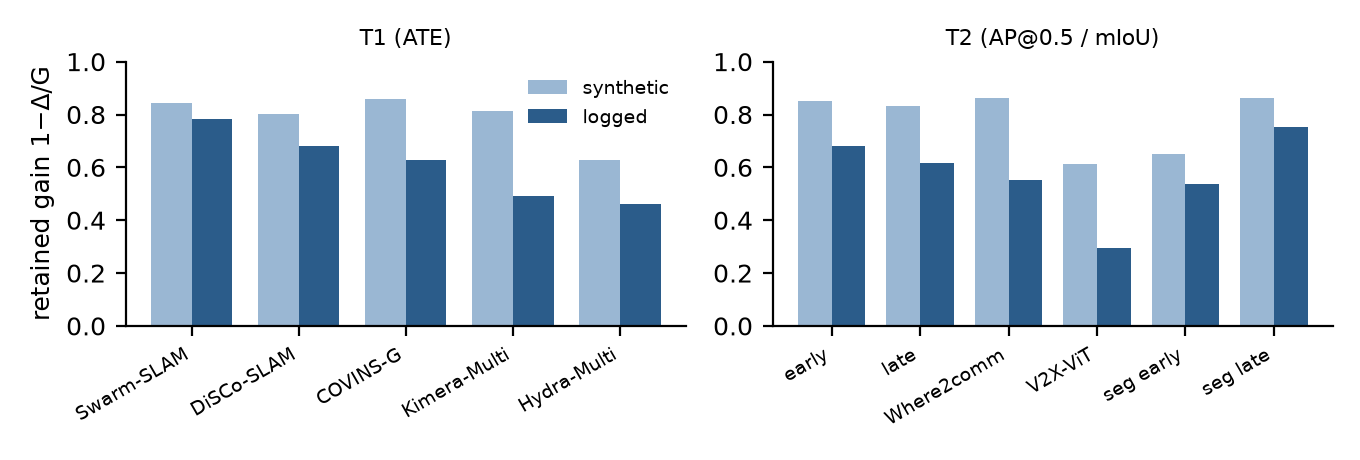
\includegraphics[width=0.9\textwidth]{figs/fig16_q1_retained.png}
\caption{Retained cooperative gain $1-\Delta/G$ per baseline under
the synthetic and logged channels. \todo{Replace dummy data.}}
\label{fig:q1}
\end{figure*}


\todo{Results text, in this order: (1) the retained gain per task;
(2) T1: which exchange pattern retained most, and whether DiSCo-SLAM
on two agents outperformed Swarm-SLAM on three; (3) T1 semantic rows:
Kimera-Multi label accuracy against Hydra-Multi, which locates the
semantic loss in alignment or in the exchanged content; (4) T2: which
message size survived, and whether the ideal-channel ranking of
fusion methods held under the logged channel; (5) T2 boxes against
labels, which separates misplaced objects from lost coverage; (6)
synthetic against logged, where the impairment model over- or
under-stated the cost; (7) T2 on T1 poses (table in the appendix),
the added loss from degraded localization; (8) the
clearance-against-RSSI check of Sec.~\ref{sec:environments}.}

\subsection{Results: What the Map Could Foresee}
\label{sec:q2}
For each frame $t$ of a logged run, the loss
$\delta_t = A_{\mathrm{ideal},t} - A_{\mathrm{logged},t}$ is the
regression target. For T2 it is the drop in recall at IoU 0.3, 0.5,
and 0.7 and the drop in mIoU at that frame; for T1 it is the increase
in translation error over the exchange window that contains $t$.
Three predictor sets are regressed on it. $\mathcal{D}$ contains the
ego-to-helper distance alone, which is the baseline available to any
team. $\mathcal{G}$ contains the map geometry of
Sec.~\ref{sec:paradigms}: $\mathrm{clear}(e,j^\star)$, link length,
$\omega_e$, $\beta$, $C$, and ego-to-object range, all computed from
the map and the poses before any signal is observed.
$\mathcal{G}\cup\mathcal{L}$ adds the measured link at $t$: goodput,
RTT, retries, and RSSI. The regressor is gradient-boosted trees
\todo{LightGBM}, fitted on two sites and evaluated on the third, over
all three folds. The anticipated share is
$R^2_{\mathcal{G}} / R^2_{\mathcal{G}\cup\mathcal{L}}$ on the held-out
site, that is, the fraction of the predictable loss that the map
alone predicts in a building on which it was not fitted
(Fig.~\ref{fig:q2}). \todo{Results: share per site and per task;
whether $\mathcal{G}$ outperformed $\mathcal{D}$; feature ablation
(appendix); one qualitative sequence with predicted and actual loss
over time. Position against map-based link prediction work.}

\begin{figure*}[t]
\centering
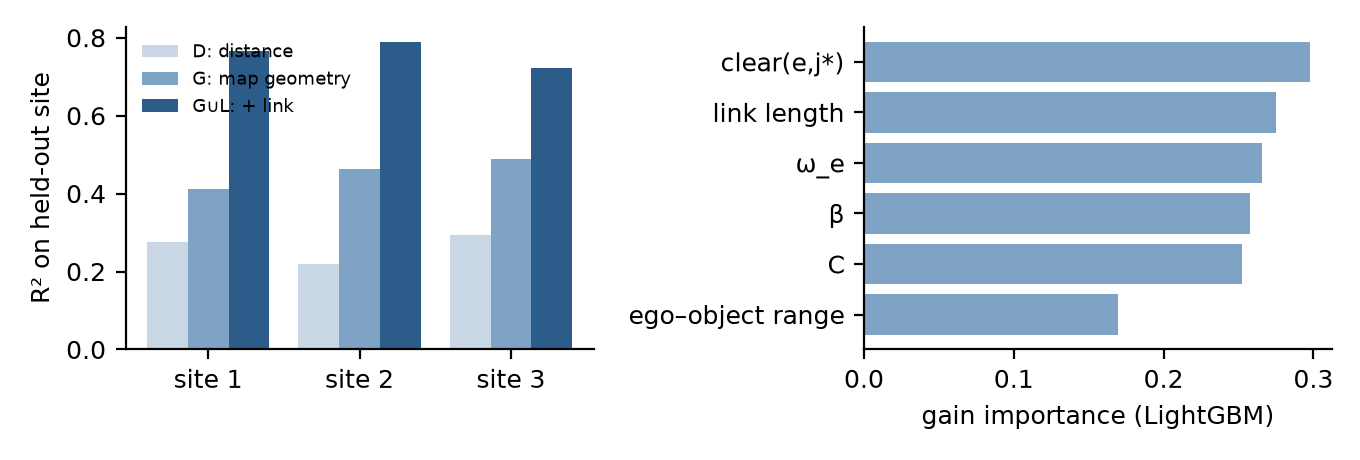
\includegraphics[width=0.9\textwidth]{figs/fig17_q2_share.png}
\caption{Left: $R^2$ of each predictor set on the held-out site.
Right: feature importance within $\mathcal{G}$. \todo{Replace dummy
data.}}
\label{fig:q2}
\end{figure*}


\subsection{Failure Cases}
\label{sec:failures}
Four sequences are shown in Fig.~\ref{fig:failures}, each with the
ego frame, the link trace, and the geometry over the same window.
Three were selected where a baseline lost most of its gain under the
logged channel: \todo{(1) a link-stress frame where the clearance
dropped below 0.6 and early fusion lost the partner's cloud; (2) an
occlusion$\times$link frame where the message of the only helper
arrived late and the box landed beyond IoU 0.7; (3) a rendezvous that
Swarm-SLAM missed because the link was down at the meeting}. The
fourth was selected where the link was intact and the baseline
failed regardless: \todo{(4) a frame with clear line of sight and
full goodput where the detector missed a small object at range}. The
fourth case shows that the benchmark attributes loss to the link only
where the link caused it.

\begin{figure*}[t]
\centering
\fbox{\parbox[c][5cm][c]{0.95\textwidth}{\centering
\todo{Fig.~18: failure cases, one column per case. Row 1: ego image
and LiDAR with predicted and ground-truth boxes. Row 2: goodput and
RTT over the window. Row 3: clearance and $\omega_e$ over the
window.}}}
\caption{Failure cases. Three where the logged link removed the
cooperative gain, one where it did not.}
\label{fig:failures}
\end{figure*}


%=======================================================================
\section{Discussion}
\label{sec:discussion}

\subsection{What the Link Costs}
\label{sec:findings}
\todo{Answer Q1 in one sentence first: how much of the cooperative
gain survives the logged link, per task.
Then discuss:
(1) Which task lost more, C-SLAM or detection, and why: C-SLAM sends
    little but needs its rare messages to arrive; detection sends every
    frame and needs them to arrive on time.
(2) Which message size survived: early, intermediate, or late fusion.
    Does the ranking of fusion methods under the ideal channel hold
    under the logged one?
(3) Synthetic versus logged: did the synthetic channel over- or
    under-state the cost, and where? Real losses are bursty and
    correlated with position, which a random-loss model misses.
(4) T2 on T1 poses: how much extra loss comes from the link degrading
    localization, compared with the link delaying perception data.}

\subsection{What the Map Could Foresee}
\todo{Answer Q2 in one sentence first: the anticipated share, and
whether geometry beat distance alone.
Then discuss, depending on the outcome:
- High share: which geometric features carried it (from the feature
  ablation), and what a team could do with it: plan routes and
  rendezvous around low clearance, send less when a link is predicted
  to fail.
- Low share: what the map misses. Candidates: people and other
  moving obstacles not in the static map, interference from other
  networks, multipath the clearance test cannot see, contention
  between agents. Check whether the unexplained loss clusters in
  time (moving obstacles, contention) or in space (propagation).
- Either way: did the predictor transfer to the held-out site? If
  not, geometry predicts link loss only in buildings it was fit on.}

\subsection{What the Characterization Shows}
\todo{Observations from the geometry itself, independent of the
benchmark. Candidates to check once sequences exist:
(1) whether range or occlusion limits the team more (visible vs.\
observed by range bin);
(2) how much the evidence definition (LiDAR vs.\ depth) changes
collaboration rates;
(3) whether elevated infrastructure is complementary for every ego, or
only depending on where the ego stands ($\beta$ per ego);
(4) whether planned paradigms produced the intended conditions
(\texttt{intended\_paradigm} vs.\ measured);
(5) whether map clearance agrees with measured RSSI.}

\subsection{Limitations}
\todo{Keep to limits that bound the claims:
- Scale: three sites, number of sequences, static vs. dynamic objects.
- Radio: one band, one protocol (802.11ac, single stream), one access
  point per site; CSI from one receiver, valid below about
  \SI{1.2}{\metre\per\second}.
- Reference: self-built map; the two passes share sensor and pipeline,
  so absolute accuracy rests on the control distances.
- Geometry: endpoint clearances hide obstacles near the radios; link
  paradigms not yet in the classifier, if still true.}

\subsection{Broader Impact and Ethics}
\todo{- Anonymisation of camera streams (faces blurred, reviewed).
- CSI can detect and localise people who appear in no camera: state
  consent, pseudonymisation of network identifiers, and a license
  clause against re-identification.
- Positive use: communication-aware planning for robots in buildings
  where infrastructure is limited, e.g. search and rescue.}

%=======================================================================
\section{Conclusion and Future Work}
\label{sec:conclusion}
We presented SCooP, a multi-agent dataset that jointly captures
synchronized sensing, cooperative perception labels, and measured
communication, with dense reconstruction supervision and benchmarks across
the three layers. \todo{One sentence of headline findings.} Future work
includes scaling to larger teams, adding modalities, and richer channel
models.

\section*{Acknowledgment}
% Optional; delete if unused. Sponsor acknowledgments go in the unnumbered
% footnote on the first page (\thanks in \title).
\todo{Add acknowledgments or delete this section.}

\bibliographystyle{IEEEtran}
\bibliography{references}

\appendices
\section{Sequence Inventory}
\label{app:sequences}
\todo{Per-sequence table: identifier, site, session, intended
paradigm, duration, distance per agent, frames, annotated instances,
median goodput and RTT per link, fraction of frames with
$\mathrm{clear} < 0.6$.}

\begin{figure*}[t]
\centering
\fbox{\parbox[c][5cm][c]{0.95\textwidth}{\centering
\todo{Fig.~20: per-sequence trajectories on each site.}}}
\caption{Trajectories of every sequence, one panel per site.}
\label{fig:app_trajectories}
\end{figure*}


\section{Sensor Intrinsics}
\label{app:intrinsics}
\todo{Per-sensor intrinsic parameters and the plots behind
Table~\ref{tab:calib}: camera reprojection residual by image region,
LiDAR range bias by range, radar reflector offset by range.}

\begin{figure}[t]
\centering
\fbox{\parbox[c][4cm][c]{0.95\columnwidth}{\centering
\todo{Fig.~19: per-sensor intrinsic calibration plots.}}}
\caption{Intrinsic calibration residuals per sensor.}
\label{fig:app_intrinsics}
\end{figure}


\section{Extended Benchmark Results}
\label{app:results}
\todo{T2 precision-recall curves at each IoU threshold per baseline
and channel; T2 results with partner data placed by T1 poses;
per-class mIoU; Q2 feature ablation, one feature removed at a time,
per site.}

\begin{figure*}[t]
\centering
\fbox{\parbox[c][5cm][c]{0.95\textwidth}{\centering
\todo{Fig.~21: T2 precision-recall at IoU 0.3, 0.5, 0.7 per baseline
and channel.}}}
\caption{Precision-recall curves for T2 at each IoU threshold.}
\label{fig:app_pr}
\end{figure*}


\begin{figure}[t]
\centering
\fbox{\parbox[c][4cm][c]{0.95\columnwidth}{\centering
\todo{Fig.~22: Q2 feature ablation, one feature removed at a time,
per site.}}}
\caption{Q2 feature ablation.}
\label{fig:app_ablation}
\end{figure}


\end{document}
